\begin{apendicesenv}

\partapendices

\chapter{Repositório do Projeto - GitHub}
\label{repositorio}

Para manter a organização, versionamento e divulgação do projeto, foi criada a organização no GitHub \href{https://github.com/Ground-Station}{Ground Station}.

\section{\href{https://github.com/Ground-Station/Documentation}{Documentação do Projeto}}

O repositório de Documentação do projeto, é responsável por manter os relatórios e manuais do projeto. 
 
\section{\href{https://github.com/Ground-Station/backend}{Backend}}

\begin{itemize}
    \item \href{https://github.com/Ground-Station/backend/tree/main/src/datasources}{banco de dados};  
    \item \href{https://github.com/Ground-Station/backend/pull/2/files}{manter hardware}; 
    \item \href{https://github.com/Ground-Station/backend/pull/1/files}{manter foguete}; 
    \item \href{https://github.com/Ground-Station/backend/pull/3/files}{configuração do ambiente};
    \item \href{https://github.com/Ground-Station/backend/pull/5/files}{Comunicação Serial entre Hardware e Software};
    \item \href{https://github.com/Ground-Station/backend/pull/4/files}{Cálculo da velocidade do foguete}.
\end{itemize} 
\section{\href{https://github.com/Ground-Station/frontend}{Frontend}}

\begin{itemize} 
    \item \href{https://github.com/Ground-Station/frontend/tree/material/ground-station/src/views/Rocket}{Manter Foguetes};
    \item \href{https://github.com/Ground-Station/frontend/tree/material/ground-station/src/views/Mission}{Manter componentes das fases da missão};
    \item \href{https://github.com/Ground-Station/frontend/tree/material/ground-station/src/views/Mission/MissionData}{Componentes dos dados expostos durante a execução de uma missão e no histórico da missão};
    \item \href{https://github.com/Ground-Station/frontend/tree/material/ground-station/src/views/Hardware}{Manter hardwares e comandos de hardware}.
\end{itemize}

\chapter{Documentação da API}
\label{documentacao_api}

\section{Foguete}
\begin{table}[H]
\begin{tabular}{|l|l|}
\hline
\textbf{Endpoint}            & /foguetes/{id} \\ \hline
\textbf{Método HTTP}         & PUT \\ \hline
\textbf{Schema}              &  
\begin{lstlisting}
{
nome*	string
pesoVazio*	number
pesoCheio*	number
id	number
}
\end{lstlisting}\\ \hline
\textbf{Exemplo Requisição}  &  
\begin{lstlisting}
{
  "nome": "string",
  "pesoVazio": 0,
  "pesoCheio": 0,
  "id": 0
}
\end{lstlisting}
\\ \hline
\textbf{Resposta de Sucesso} & 
\begin{lstlisting}
{
"status": "204",
"description": "Foguete PUT success"
}
\end{lstlisting}
\\ \hline
\textbf{Resposta de Erro}    &  \\ \hline
\end{tabular}
\caption{PUT foguetes.}
\label{put_foguetes}
\end{table}

\begin{table}[H]
\begin{tabular}{|l|l|}
\hline
\textbf{Endpoint}            & /foguetes/{id} \\ \hline
\textbf{Método HTTP}         & PATCH \\ \hline
\textbf{Schema}              &  
\begin{lstlisting}
{
nome*	string
pesoVazio*	number
pesoCheio*	number
id	number
}
\end{lstlisting}\\ \hline
\textbf{Exemplo Requisição}  &  
\begin{lstlisting}
{
  "nome": "string",
  "pesoVazio": 0,
  "pesoCheio": 0,
  "id": 0
}
\end{lstlisting}
\\ \hline
\textbf{Resposta de Sucesso} &
\begin{lstlisting}
{
"status": "204",
"description": "Foguete PATCH success"
}
\end{lstlisting}
\\ \hline
\textbf{Resposta de Erro}    &  \\ \hline
\end{tabular}
\caption{PATCH foguetes.}
\label{patch_foguetes}
\end{table}

\begin{table}[H]
\begin{tabular}{|l|l|}
\hline
\textbf{Endpoint}            & /foguetes/{id} \\ \hline
\textbf{Método HTTP}         & GET \\ \hline
\textbf{Schema}              &  
\begin{lstlisting}
{
nome*	string
pesoVazio*	number
pesoCheio*	number
id	number
}
\end{lstlisting}\\ \hline
\textbf{Exemplo Requisição}  &  -- \\ \hline
\textbf{Resposta de Sucesso} &
\begin{lstlisting}
{
"status": "200",
"description": "Foguete model instance"
}
{
  "nome": "string",
  "pesoVazio": 0,
  "pesoCheio": 0,
  "id": 0
}
\end{lstlisting}
\\ \hline
\textbf{Resposta de Erro}    &  \\ \hline
\end{tabular}
\caption{GET foguetes pelo ID.}
\label{get_foguetes_id}
\end{table}

\begin{table}[H]
\begin{tabular}{|l|l|}
\hline
\textbf{Endpoint}            & /foguetes/{id} \\ \hline
\textbf{Método HTTP}         & DELETE \\ \hline
\textbf{Schema}              &  -- \\ \hline
\textbf{Exemplo Requisição}  &  -- \\ \hline
\textbf{Resposta de Sucesso} &
\begin{lstlisting}
{
"status": "204",
"description": "Foguete DELETE success"
}
\end{lstlisting}
\\ \hline
\textbf{Resposta de Erro}    &  \\ \hline
\end{tabular}
\caption{DELETE foguetes.}
\label{delete_foguetes}
\end{table}


\begin{table}[H]
\begin{tabular}{|l|l|}
\hline
\textbf{Endpoint}            & /foguetes \\ \hline
\textbf{Método HTTP}         & POST \\ \hline
\textbf{Schema}              &  
\begin{lstlisting}
{
nome*	string
pesoVazio*	number
pesoCheio*	number
}
\end{lstlisting}\\ \hline
\textbf{Exemplo Requisição}  &  
\begin{lstlisting}
{
  "nome": "string",
  "pesoVazio": 0,
  "pesoCheio": 0
}
\end{lstlisting}
\\ \hline
\textbf{Resposta de Sucesso} &
\begin{lstlisting}
{
"status": "200",
"description": "Foguete model instance"
}
{
  "nome": "string",
  "pesoVazio": 0,
  "pesoCheio": 0,
  "id": 0
}
\end{lstlisting}
\\ \hline
\textbf{Resposta de Erro}    &  \\ \hline
\end{tabular}
\caption{POST foguetes.}
\label{post_foguetes}
\end{table}

\begin{table}[H]
\begin{tabular}{|l|l|}
\hline
\textbf{Endpoint}            & /foguetes \\ \hline
\textbf{Método HTTP}         & GET \\ \hline
\textbf{Schema}              &  
\begin{lstlisting}
{
nome*	string
pesoVazio*	number
pesoCheio*	number
id	number
}
\end{lstlisting}\\ \hline
\textbf{Exemplo Requisição}  &  -- \\ \hline
\textbf{Resposta de Sucesso} &
\begin{lstlisting}
{
"status": "200",
"description": "Array of Foguete model instances"
}
[
  {
    "nome": "string",
    "pesoVazio": 0,
    "pesoCheio": 0,
    "id": 0
  },
  {
    "nome": "string",
    "pesoVazio": 0,
    "pesoCheio": 0,
    "id": 0
  },
]
\end{lstlisting}
\\ \hline
\textbf{Resposta de Erro}    &  \\ \hline
\end{tabular}
\caption{GET foguetes.}
\label{get_foguetes}
\end{table}

\section{Hardware}
%#######################################################
\begin{table}[H]
\begin{tabular}{|l|l|}
\hline
\textbf{Endpoint}            & /hardware \\ \hline
\textbf{Método HTTP}         & POST \\ \hline
\textbf{Schema}              & 
\begin{lstlisting}
{
nomeHardware*	string
baudRate*	number
portaSerial*	string
}
\end{lstlisting}
\\ \hline
\textbf{Exemplo Requisição}  &  
\begin{lstlisting}
{
  "nomeHardware": "string",
  "baudRate": 0,
  "portaSerial": "string"
}
\end{lstlisting}
\\ \hline
\textbf{Resposta de Sucesso} & 
\begin{lstlisting}
{
"status": "200",
"description": "Hardware model instance"
}
{
  "id": "string",
  "nomeHardware": "string",
  "baudRate": 0,
  "portaSerial": "string"
}
\end{lstlisting}
\\ \hline
\end{tabular}
\caption{POST hardware.}
\label{post_hardware}
\end{table}
%#######################################################
\begin{table}[H]
\begin{tabular}{|l|l|}
\hline
\textbf{Endpoint}            & /hardware/{id} \\ \hline
\textbf{Método HTTP}         & DELETE \\ \hline
\textbf{Schema}              &  -- \\ \hline
\textbf{Exemplo Requisição}  &  -- \\ \hline
\textbf{Resposta de Sucesso} &
\begin{lstlisting}
{
"status": "204",
"description": "Hardware DELETE success"
}
\end{lstlisting}
\\ \hline
\textbf{Resposta de Erro}    &  \\ \hline
\end{tabular}
\caption{DELETE hardware.}
\label{delete_hardware}
\end{table}
%#######################################################
\begin{table}[H]
\begin{tabular}{|l|l|}
\hline
\textbf{Endpoint}            & /hardware \\ \hline
\textbf{Método HTTP}         & GET \\ \hline
\textbf{Schema}              & -- \\ \hline
\textbf{Exemplo Requisição}  & -- \\ \hline
\textbf{Resposta de Sucesso} & 
\begin{lstlisting}
{
"status": "200",
"description": "Array of Hardware model instances"
}
[
  {
    "id": "string",
    "nomeHardware": "string",
    "baudRate": 0,
    "portaSerial": "string",
    "hardwareComandos": [
      {
        "id": "string",
        "nome": "string",
        "valor": 0
      }
    ]
  }
]
\end{lstlisting}
\\ \hline
\end{tabular}
\caption{GET hardware.}
\label{get_hardware}
\end{table}
%#######################################################


\section{Comandos}

\begin{table}[H]
\begin{tabular}{|l|l|}
\hline
\textbf{Endpoint}            & /comandos/{id} \\ \hline
\textbf{Método HTTP}         & PUT \\ \hline
\textbf{Schema}              &  
\begin{lstlisting}
{
id	string
nome*	string
valor*	number
}
\end{lstlisting}\\ \hline
\textbf{Exemplo Requisição}  &  
\begin{lstlisting}
{
  "id": "string",
  "nome": "string",
  "valor": 0
}
\end{lstlisting} \\ \hline
\textbf{Resposta de Sucesso} &
\begin{lstlisting}
{
"status": "204",
"description": "Comando PUT success"
}
\end{lstlisting}
\\ \hline
\end{tabular}
\caption{PUT comandos.}
\label{put_comandos}
\end{table}

%#######################################################

\begin{table}[H]
\begin{tabular}{|l|l|}
\hline
\textbf{Endpoint}            & /comandos/{id} \\ \hline
\textbf{Método HTTP}         & PATCH \\ \hline
\textbf{Schema}              &  
\begin{lstlisting}
{
id	string
nome*	string
valor*	number
}
\end{lstlisting}\\ \hline
\textbf{Exemplo Requisição}  &  
\begin{lstlisting}
{
  "id": "string",
  "nome": "string",
  "valor": 0
}
\end{lstlisting} \\ \hline
\textbf{Resposta de Sucesso} &
\begin{lstlisting}
{
"status": "204",
"description": "Comando PATCH success"
}
\end{lstlisting}
\\ \hline
\end{tabular}
\caption{PATCH comandos.}
\label{patch_comandos}
\end{table}

%#######################################################

\begin{table}[H]
\begin{tabular}{|l|l|}
\hline
\textbf{Endpoint}            & /comandos/{id} \\ \hline
\textbf{Método HTTP}         & GET \\ \hline
\textbf{Schema}              & -- \\ \hline
\textbf{Exemplo Requisição}  & -- \\ \hline
\textbf{Resposta de Sucesso} &
\begin{lstlisting}
{
"status": "200",
"description": "Comando model instance"
}
{
  "id": "string",
  "nome": "string",
  "valor": 0
}
\end{lstlisting}
\\ \hline
\end{tabular}
\caption{GET comandos pelo ID.}
\label{get_comandos_id}
\end{table}

%#######################################################

\begin{table}[H]
\begin{tabular}{|l|l|}
\hline
\textbf{Endpoint}            & /comandos/{id} \\ \hline
\textbf{Método HTTP}         & DELETE \\ \hline
\textbf{Schema}              & -- \\ \hline
\textbf{Exemplo Requisição}  & -- \\ \hline
\textbf{Resposta de Sucesso} &
\begin{lstlisting}
{
"status": "204",
"description": "Comando DELETE sucess"
}
\end{lstlisting}
\\ \hline
\end{tabular}
\caption{DELETE comandos.}
\label{delete_comandos}
\end{table}

%#######################################################

\begin{table}[H]
\begin{tabular}{|l|l|}
\hline
\textbf{Endpoint}            & /comandos \\ \hline
\textbf{Método HTTP}         & POST \\ \hline
\textbf{Schema}              & 
\begin{lstlisting}
{
nome*	string
valor*	number
}
\end{lstlisting} \\ \hline
\textbf{Exemplo Requisição}  & 
\begin{lstlisting}
{
  "nome": "string",
  "valor": 0
}
\end{lstlisting} \\ \hline
\textbf{Resposta de Sucesso} &
\begin{lstlisting}
{
"status": "200",
"description": "Comando model instance"
}
{
  "id": "string",
  "nome": "string",
  "valor": 0
}
\end{lstlisting}
\\ \hline
\end{tabular}
\caption{POST comandos.}
\label{post_comandos}
\end{table}

%#######################################################

\begin{table}[H]
\begin{tabular}{|l|l|}
\hline
\textbf{Endpoint}            & /comandos \\ \hline
\textbf{Método HTTP}         & GET \\ \hline
\textbf{Schema}              & 
\begin{lstlisting}
{
id	string
nome*	string
valor*	number
}
\end{lstlisting} \\ \hline
\textbf{Exemplo Requisição}  & -- \\ \hline
\textbf{Resposta de Sucesso} &
\begin{lstlisting}
{
"status": "200",
"description": "Array of Comando model instances"
}
[
    {
      "id": "string",
      "nome": "string",
      "valor": 0
    },
    {
      "id": "string",
      "nome": "string",
      "valor": 0
    }
]
\end{lstlisting} \\ \hline
\end{tabular}
\caption{GET comandos.}
\label{get_comandos}
\end{table}

%#######################################################

\section{Missão}

\begin{table}[H]
\begin{tabular}{|l|l|}
\hline
\textbf{Endpoint}            & /missao/{id} \\ \hline
\textbf{Método HTTP}         & PUT \\ \hline
\textbf{Schema}              &  
\begin{lstlisting}
{
id	string
apogeuEsperado*	number
nomeMissao*	string
}
\end{lstlisting}\\ \hline
\textbf{Exemplo Requisição}  &  
\begin{lstlisting}
{
  "id": "string",
  "apogeuEsperado": 0,
  "nomeMissao": "string"
}
\end{lstlisting} \\ \hline
\textbf{Resposta de Sucesso} &
\begin{lstlisting}
{
"status": "204",
"description": "Missao PUT success"
}
\end{lstlisting}
\\ \hline
\end{tabular}
\caption{PUT  missao pelo ID.}
\label{put_missao}
\end{table}

%#######################################################

\begin{table}[H]
\begin{tabular}{|l|l|}
\hline
\textbf{Endpoint}            & /missao/{id} \\ \hline
\textbf{Método HTTP}         & PATCH \\ \hline
\textbf{Schema}              &  
\begin{lstlisting}
{
id	string
nome*	string
valor*	number
}
\end{lstlisting}\\ \hline
\textbf{Exemplo Requisição}  &  
\begin{lstlisting}
{
  "id": "string",
  "apogeuEsperado": 0,
  "nomeMissao": "string"
}
\end{lstlisting} \\ \hline
\textbf{Resposta de Sucesso} &
\begin{lstlisting}
{
"status": "204",
"description": "Missao PATCH success"
}
\end{lstlisting}
\\ \hline
\end{tabular}
\caption{PATCH missão.}
\label{patch_missao}
\end{table}

%#######################################################

\begin{table}[H]
\begin{tabular}{|l|l|}
\hline
\textbf{Endpoint}            & /missao/{id} \\ \hline
\textbf{Método HTTP}         & GET \\ \hline
\textbf{Schema}              & -- \\ \hline
\textbf{Exemplo Requisição}  & -- \\ \hline
\textbf{Resposta de Sucesso} &
\begin{lstlisting}
{
"status": "200",
"description": "Missao model instance"
}
{
  "id": "string",
  "apogeuEsperado": 0,
  "nomeMissao": "string"
}
\end{lstlisting}
\\ \hline
\end{tabular}
\caption{GET missão pelo ID.}
\label{get_missao_id}
\end{table}

%#######################################################

\begin{table}[H]
\begin{tabular}{|l|l|}
\hline
\textbf{Endpoint}            & /missao/{id} \\ \hline
\textbf{Método HTTP}         & DELETE \\ \hline
\textbf{Schema}              & -- \\ \hline
\textbf{Exemplo Requisição}  & -- \\ \hline
\textbf{Resposta de Sucesso} &
\begin{lstlisting}
{
"status": "204",
"description": "Missao DELETE success"
}
\end{lstlisting}
\\ \hline
\end{tabular}
\caption{DELETE missão.}
\label{delete_missao}
\end{table}

%#######################################################

\begin{table}[H]
\begin{tabular}{|l|l|}
\hline
\textbf{Endpoint}            & /missao \\ \hline
\textbf{Método HTTP}         & POST \\ \hline
\textbf{Schema}              & 
\begin{lstlisting}
{
apogeuEsperado*	number
nomeMissao*	string
}
\end{lstlisting} \\ \hline
\textbf{Exemplo Requisição}  & 
\begin{lstlisting}
{
  "apogeuEsperado": 0,
  "nomeMissao": "string"
}
\end{lstlisting} \\ \hline
\textbf{Resposta de Sucesso} &
\begin{lstlisting}
{
"status": "200",
"description": "Missao model instance"
}
{
  "id": "string",
  "apogeuEsperado": 0,
  "nomeMissao": "string"
}
\end{lstlisting}
\\ \hline
\end{tabular}
\caption{POST missão.}
\label{post_missao}
\end{table}

%#######################################################

\begin{table}[H]
\begin{tabular}{|l|l|}
\hline
\textbf{Endpoint}            & /missao \\ \hline
\textbf{Método HTTP}         & GET \\ \hline
\textbf{Schema}              & 
\begin{lstlisting}
{
id	string
apogeuEsperado*	number
nomeMissao*	string
}
\end{lstlisting} \\ \hline
\textbf{Exemplo Requisição}  & -- \\ \hline
\textbf{Resposta de Sucesso} &
\begin{lstlisting}
{
"status": "200",
"description": "Array of Missao model instances"
}
[
  {
    "id": "string",
    "apogeuEsperado": 0,
    "nomeMissao": "string"
  },
  {
    "id": "string",
    "apogeuEsperado": 0,
    "nomeMissao": "string"
  }
]
\end{lstlisting} \\ \hline
\end{tabular}
\caption{GET missões.}
\label{get_missao}
\end{table}

%#######################################################

\section{Dados coletados}

\subsection{GPS}

\begin{table}[H]
\begin{tabular}{|l|l|}
\hline
\textbf{Endpoint}            & /gps/{id} \\ \hline
\textbf{Método HTTP}         & PUT \\ \hline
\textbf{Schema}              &  
\begin{lstlisting}
{
latitude*	number
longitude*	number
id	string
}
\end{lstlisting}\\ \hline
\textbf{Exemplo Requisição}  &  
\begin{lstlisting}
{
  "latitude": 0,
  "longitude": 0,
  "id": "string",
}
\end{lstlisting} \\ \hline
\textbf{Resposta de Sucesso} &
\begin{lstlisting}
{
"status": "204",
"description": "Gps PUT success"
}
\end{lstlisting}
\\ \hline
\end{tabular}
\caption{PUT GPS.}
\label{put_gps}
\end{table}

%#######################################################

\begin{table}[H]
\begin{tabular}{|l|l|}
\hline
\textbf{Endpoint}            & /gps/{id} \\ \hline
\textbf{Método HTTP}         & PATCH \\ \hline
\textbf{Schema}              &  
\begin{lstlisting}
{
latitude*	number
longitude*	number
id	string
}
\end{lstlisting}\\ \hline
\textbf{Exemplo Requisição}  &  
\begin{lstlisting}
{
  "latitude": 0,
  "longitude": 0,
  "id": "string",
}
\end{lstlisting} \\ \hline
\textbf{Resposta de Sucesso} &
\begin{lstlisting}
{
"status": "204",
"description": "Gps PATCH success"
}
\end{lstlisting}
\\ \hline
\end{tabular}
\caption{PATCH GPS pelo ID.}
\label{patch_gps_id}
\end{table}

%#######################################################

\begin{table}[H]
\begin{tabular}{|l|l|}
\hline
\textbf{Endpoint}            & /gps/{id} \\ \hline
\textbf{Método HTTP}         & GET \\ \hline
\textbf{Schema}              & -- \\ \hline
\textbf{Exemplo Requisição}  & -- \\ \hline
\textbf{Resposta de Sucesso} &
\begin{lstlisting}
{
"status": "200",
"description": "Gps model instance"
}
{
  "latitude": 0,
  "longitude": 0,
  "id": "string"
}
\end{lstlisting}
\\ \hline
\end{tabular}
\caption{GET GPS pelo ID.}
\label{get_gps_id}
\end{table}

%#######################################################

\begin{table}[H]
\begin{tabular}{|l|l|}
\hline
\textbf{Endpoint}            & /gps/{id} \\ \hline
\textbf{Método HTTP}         & DELETE \\ \hline
\textbf{Schema}              & -- \\ \hline
\textbf{Exemplo Requisição}  & -- \\ \hline
\textbf{Resposta de Sucesso} &
\begin{lstlisting}
{
"status": "204",
"description": "Gps DELETE success"
}
\end{lstlisting}
\\ \hline
\end{tabular}
\caption{GET GPS pelo ID.}
\label{delete_gps}
\end{table}

%#######################################################

\begin{table}[H]
\begin{tabular}{|l|l|}
\hline
\textbf{Endpoint}            & /gps \\ \hline
\textbf{Método HTTP}         & POST \\ \hline
\textbf{Schema}              & 
\begin{lstlisting}
{
latitude*	number
longitude*	number
}
\end{lstlisting} \\ \hline
\textbf{Exemplo Requisição}  & 
\begin{lstlisting}
{
  "latitude": 0,
  "longitude": 0
}
\end{lstlisting} \\ \hline
\textbf{Resposta de Sucesso} &
\begin{lstlisting}
{
"status": "200",
"description": "Gps model instance"
}
{
  "latitude": 0,
  "longitude": 0,
  "id": "string"
}
\end{lstlisting}
\\ \hline
\end{tabular}
\caption{POST GPS.}
\label{post_gps}
\end{table}

%#######################################################

\begin{table}[H]
\begin{tabular}{|l|l|}
\hline
\textbf{Endpoint}            & /gps \\ \hline
\textbf{Método HTTP}         & GET \\ \hline
\textbf{Schema}              & 
\begin{lstlisting}
{
latitude*	number
longitude*	number
}
\end{lstlisting} \\ \hline
\textbf{Exemplo Requisição}  & -- \\ \hline
\textbf{Resposta de Sucesso} &
\begin{lstlisting}
{
"status": "200",
"description": "Array of Missao model instances"
}
[
  {
    "latitude": 0,
    "longitude": 0,
    "id": "string"
  },
  {
    "latitude": 0,
    "longitude": 0,
    "id": "string"
  }
]
\end{lstlisting} \\ \hline
\end{tabular}
\caption{GET GPS.}
\label{get_gps}
\end{table}

%#######################################################
\subsection{Peso}

\begin{table}[H]
\begin{tabular}{|l|l|}
\hline
\textbf{Endpoint}            & /pesos/{id} \\ \hline
\textbf{Método HTTP}         & PUT \\ \hline
\textbf{Schema}              &  
\begin{lstlisting}
{
peso*	number
tempo*	string($date-time)
id	string
}
\end{lstlisting}\\ \hline
\textbf{Exemplo Requisição}  &  
\begin{lstlisting}
{
  "peso": 0,
  "tempo": "2020-11-22T20:04:33.198Z",
  "id": "string"
}
\end{lstlisting} \\ \hline
\textbf{Resposta de Sucesso} &
\begin{lstlisting}
{
"status": "204",
"description": "Peso PUT success"
}
\end{lstlisting}
\\ \hline
\end{tabular}
\caption{PUT peso.}
\label{put_peso}
\end{table}

%#######################################################

\begin{table}[H]
\begin{tabular}{|l|l|}
\hline
\textbf{Endpoint}            & /pesos/{id} \\ \hline
\textbf{Método HTTP}         & PATCH \\ \hline
\textbf{Schema}              &  
\begin{lstlisting}
{
peso*	number
tempo*	string($date-time)
id	string
}
\end{lstlisting}\\ \hline
\textbf{Exemplo Requisição}  &  
\begin{lstlisting}
{
  "peso": 0,
  "tempo": "2020-11-22T20:04:33.198Z",
  "id": "string"
}
\end{lstlisting} \\ \hline
\textbf{Resposta de Sucesso} &
\begin{lstlisting}
{
"status": "204",
"description": "Peso PATCH success"
}
\end{lstlisting}
\\ \hline
\end{tabular}
\caption{PATCH peso.}
\label{patch_peso}
\end{table}

%#######################################################

\begin{table}[H]
\begin{tabular}{|l|l|}
\hline
\textbf{Endpoint}            & /pesos/{id} \\ \hline
\textbf{Método HTTP}         & GET \\ \hline
\textbf{Schema}              & -- \\ \hline
\textbf{Exemplo Requisição}  & -- \\ \hline
\textbf{Resposta de Sucesso} &
\begin{lstlisting}
{
"status": "200",
"description": "Peso model instance"
}
{
  "peso": 0,
  "tempo": "2020-11-22T20:06:56.113Z",
  "id": "string"
}
\end{lstlisting}
\\ \hline
\end{tabular}
\caption{GET peso pelo ID.}
\label{get_peso_id}
\end{table}

%#######################################################

\begin{table}[H]
\begin{tabular}{|l|l|}
\hline
\textbf{Endpoint}            & /pesos/{id} \\ \hline
\textbf{Método HTTP}         & DELETE \\ \hline
\textbf{Schema}              & -- \\ \hline
\textbf{Exemplo Requisição}  & -- \\ \hline
\textbf{Resposta de Sucesso} &
\begin{lstlisting}
{
"status": "204",
"description": "Peso DELETE success"
}
\end{lstlisting}
\\ \hline
\end{tabular}
\caption{DELETE peso.}
\label{delete_peso}
\end{table}

%#######################################################

\begin{table}[H]
\begin{tabular}{|l|l|}
\hline
\textbf{Endpoint}            & /pesos \\ \hline
\textbf{Método HTTP}         & POST \\ \hline
\textbf{Schema}              & 
\begin{lstlisting}
{
peso*	number
tempo*	string($date-time)
}
\end{lstlisting} \\ \hline
\textbf{Exemplo Requisição}  & 
\begin{lstlisting}
{
  "peso": 0,
  "tempo": "2020-11-22T20:07:24.779Z"
}
\end{lstlisting} \\ \hline
\textbf{Resposta de Sucesso} &
\begin{lstlisting}
{
"status": "200",
"description": "Peso model instance"
}
{
  "latitude": 0,
  "longitude": 0,
  "id": "string"
}
\end{lstlisting}
\\ \hline
\end{tabular}
\caption{POST peso.}
\label{post_peso}
\end{table}

%#######################################################

\begin{table}[H]
\begin{tabular}{|l|l|}
\hline
\textbf{Endpoint}            & /pesos \\ \hline
\textbf{Método HTTP}         & GET \\ \hline
\textbf{Schema}              & 
\begin{lstlisting}
{
peso*	number
tempo*	string($date-time)
}
\end{lstlisting} \\ \hline
\textbf{Exemplo Requisição}  & -- \\ \hline
\textbf{Resposta de Sucesso} &
\begin{lstlisting}
{
"status": "200",
"description": "Array of Peso model instances"
}
[
  {
    "peso": 0,
    "tempo": "2020-11-22T20:07:58.672Z",
    "id": "string"
  },
  {
    "peso": 0,
    "tempo": "2020-11-22T20:07:58.672Z",
    "id": "string"
  }
]
\end{lstlisting} \\ \hline
\end{tabular}
\caption{GET pesos.}
\label{get_peso}
\end{table}

%#######################################################
\subsection{Pressão}

\begin{table}[H]
\begin{tabular}{|l|l|}
\hline
\textbf{Endpoint}            & /pressao/{id} \\ \hline
\textbf{Método HTTP}         & PUT \\ \hline
\textbf{Schema}              &  
\begin{lstlisting}
{
pressao*	number
tempo*	string($date-time)
id	string
}
\end{lstlisting}\\ \hline
\textbf{Exemplo Requisição}  &  
\begin{lstlisting}
{
  "pressao": 0,
  "tempo": "2020-11-22T22:32:32.108Z",
  "id": "string"
}
\end{lstlisting} \\ \hline
\textbf{Resposta de Sucesso} &
\begin{lstlisting}
{
"status": "204",
"description": "Pressao PUT success"
}
\end{lstlisting}
\\ \hline
\end{tabular}
\caption{PUT pressão.}
\label{put_pressao}
\end{table}

%#######################################################

\begin{table}[H]
\begin{tabular}{|l|l|}
\hline
\textbf{Endpoint}            & /pressao/{id} \\ \hline
\textbf{Método HTTP}         & PATCH \\ \hline
\textbf{Schema}              &  
\begin{lstlisting}
{
pressao*	number
tempo*	string($date-time)
id	string
}
\end{lstlisting}\\ \hline
\textbf{Exemplo Requisição}  &  
\begin{lstlisting}
{
  "pressao": 0,
  "tempo": "2020-11-22T22:32:32.108Z",
  "id": "string"
}
\end{lstlisting} \\ \hline
\textbf{Resposta de Sucesso} &
\begin{lstlisting}
{
"status": "204",
"description": "Pressao PATCH success"
}
\end{lstlisting}
\\ \hline
\end{tabular}
\caption{PATCH pressão.}
\label{patch_pressao}
\end{table}

%#######################################################

\begin{table}[H]
\begin{tabular}{|l|l|}
\hline
\textbf{Endpoint}            & /pressao/{id} \\ \hline
\textbf{Método HTTP}         & GET \\ \hline
\textbf{Schema}              & -- \\ \hline
\textbf{Exemplo Requisição}  & -- \\ \hline
\textbf{Resposta de Sucesso} &
\begin{lstlisting}
{
"status": "200",
"description": "Pressao model instance"
}
{
  "pressao": 0,
  "tempo": "2020-11-22T22:32:32.108Z",
  "id": "string"
}
\end{lstlisting}
\\ \hline
\end{tabular}
\caption{GET pressão pelo ID.}
\label{get_pressao_id}
\end{table}

%#######################################################

\begin{table}[H]
\begin{tabular}{|l|l|}
\hline
\textbf{Endpoint}            & /pressao/{id} \\ \hline
\textbf{Método HTTP}         & DELETE \\ \hline
\textbf{Schema}              & -- \\ \hline
\textbf{Exemplo Requisição}  & -- \\ \hline
\textbf{Resposta de Sucesso} &
\begin{lstlisting}
{
"status": "204",
"description": "Pressao DELETE success"
}
\end{lstlisting}
\\ \hline
\end{tabular}
\caption{DELETE pressão.}
\label{delete_pressao}
\end{table}

%#######################################################

\begin{table}[H]
\begin{tabular}{|l|l|}
\hline
\textbf{Endpoint}            & /pressao \\ \hline
\textbf{Método HTTP}         & POST \\ \hline
\textbf{Schema}              & 
\begin{lstlisting}
{
pressao*	number
tempo*	string($date-time)
}
\end{lstlisting} \\ \hline
\textbf{Exemplo Requisição}  & 
\begin{lstlisting}
{
  "pressao": 0,
  "tempo": "2020-11-22T22:32:32.108Z"
}
\end{lstlisting} \\ \hline
\textbf{Resposta de Sucesso} &
\begin{lstlisting}
{
"status": "200",
"description": "Pressao model instance"
}
{
  "pressao": 0,
  "tempo": "2020-11-22T22:32:32.108Z",
  "id": "string"
}
\end{lstlisting}
\\ \hline
\end{tabular}
\caption{POST pressão.}
\label{post_pressao}
\end{table}

%#######################################################

\begin{table}[H]
\begin{tabular}{|l|l|}
\hline
\textbf{Endpoint}            & /pressao \\ \hline
\textbf{Método HTTP}         & GET \\ \hline
\textbf{Schema}              & 
\begin{lstlisting}
{
pressao*	number
tempo*	string($date-time)
}
\end{lstlisting} \\ \hline
\textbf{Exemplo Requisição}  & -- \\ \hline
\textbf{Resposta de Sucesso} &
\begin{lstlisting}
{
"status": "200",
"description": "Array of Pressao model instances"
}
[
  {
    "pressao": 0,
    "tempo": "2020-11-22T22:32:32.108Z",
    "id": "string"
  },
  {
    "pressao": 0,
    "tempo": "2020-11-22T22:32:32.108Z",
    "id": "string"
  }
]
\end{lstlisting} \\ \hline
\end{tabular}
\caption{GET pressão.}
\label{get_pressao}
\end{table}

%#######################################################
\subsection{Altitude}

\begin{table}[H]
\begin{tabular}{|l|l|}
\hline
\textbf{Endpoint}            & /altitude/{id} \\ \hline
\textbf{Método HTTP}         & PUT \\ \hline
\textbf{Schema}              &  
\begin{lstlisting}
{
altitude*	number
tempo*	string($date-time)
id	string
}
\end{lstlisting}\\ \hline
\textbf{Exemplo Requisição}  &  
\begin{lstlisting}
{
  "altitude": 0,
  "tempo": "2020-11-22T22:32:32.108Z",
  "id": "string"
}
\end{lstlisting} \\ \hline
\textbf{Resposta de Sucesso} &
\begin{lstlisting}
{
"status": "204",
"description": "Altitude PUT success"
}
\end{lstlisting}
\\ \hline
\end{tabular}
\caption{PUT altitude.}
\label{put_altitude}
\end{table}

%#######################################################

\begin{table}[H]
\begin{tabular}{|l|l|}
\hline
\textbf{Endpoint}            & /altitude/{id} \\ \hline
\textbf{Método HTTP}         & PATCH \\ \hline
\textbf{Schema}              &  
\begin{lstlisting}
{
altitude*	number
tempo*	string($date-time)
id	string
}
\end{lstlisting}\\ \hline
\textbf{Exemplo Requisição}  &  
\begin{lstlisting}
{
  "altitude": 0,
  "tempo": "2020-11-22T22:32:32.108Z",
  "id": "string"
}
\end{lstlisting} \\ \hline
\textbf{Resposta de Sucesso} &
\begin{lstlisting}
{
"status": "204",
"description": "Altitude PATCH success"
}
\end{lstlisting}
\\ \hline
\end{tabular}
\caption{PATCH altitude.}
\label{patch_altitude}
\end{table}

%#######################################################

\begin{table}[H]
\begin{tabular}{|l|l|}
\hline
\textbf{Endpoint}            & /altitude/{id} \\ \hline
\textbf{Método HTTP}         & GET \\ \hline
\textbf{Schema}              & -- \\ \hline
\textbf{Exemplo Requisição}  & -- \\ \hline
\textbf{Resposta de Sucesso} &
\begin{lstlisting}
{
"status": "200",
"description": "Altitude model instance"
}
{
  "altitude": 0,
  "tempo": "2020-11-22T22:32:32.108Z",
  "id": "string"
}
\end{lstlisting}
\\ \hline
\end{tabular}
\caption{GET altitude pelo ID.}
\label{get_altitude_id}
\end{table}

%#######################################################

\begin{table}[H]
\begin{tabular}{|l|l|}
\hline
\textbf{Endpoint}            & /altitude/{id} \\ \hline
\textbf{Método HTTP}         & DELETE \\ \hline
\textbf{Schema}              & -- \\ \hline
\textbf{Exemplo Requisição}  & -- \\ \hline
\textbf{Resposta de Sucesso} &
\begin{lstlisting}
{
"status": "204",
"description": "Altitude DELETE success"
}
\end{lstlisting}
\\ \hline
\end{tabular}
\caption{DELETE altitude.}
\label{delete_altitude}
\end{table}

%#######################################################

\begin{table}[H]
\begin{tabular}{|l|l|}
\hline
\textbf{Endpoint}            & /altitude \\ \hline
\textbf{Método HTTP}         & POST \\ \hline
\textbf{Schema}              & 
\begin{lstlisting}
{
altitude*	number
tempo*	string($date-time)
}
\end{lstlisting} \\ \hline
\textbf{Exemplo Requisição}  & 
\begin{lstlisting}
{
  "altitude": 0,
  "tempo": "2020-11-22T22:32:32.108Z"
}
\end{lstlisting} \\ \hline
\textbf{Resposta de Sucesso} &
\begin{lstlisting}
{
"status": "200",
"description": "Altitude model instance"
}
{
  "altitude": 0,
  "tempo": "2020-11-22T22:32:32.108Z",
  "id": "string"
}
\end{lstlisting}
\\ \hline
\end{tabular}
\caption{POST altitude.}
\label{post_altitude}
\end{table}

%#######################################################

\begin{table}[H]
\begin{tabular}{|l|l|}
\hline
\textbf{Endpoint}            & /altitude \\ \hline
\textbf{Método HTTP}         & GET \\ \hline
\textbf{Schema}              & 
\begin{lstlisting}
{
altitude*	number
tempo*	string($date-time)
}
\end{lstlisting} \\ \hline
\textbf{Exemplo Requisição}  & -- \\ \hline
\textbf{Resposta de Sucesso} &
\begin{lstlisting}
{
"status": "200",
"description": "Array of Altitude model instances"
}
[
  {
    "altitude": 0,
    "tempo": "2020-11-22T22:32:32.108Z",
    "id": "string"
  },
  {
    "altitude": 0,
    "tempo": "2020-11-22T22:32:32.108Z",
    "id": "string"
  }
]
\end{lstlisting} \\ \hline
\end{tabular}
\caption{GET altitude.}
\label{get_altitude}
\end{table}

%#######################################################


\chapter{Caso de Teste do Software}
\label{caso_teste_software}
\section{Manter Foguete}
\subsection{Criar foguete com sucesso}
\begin{itemize} 
    \item \textbf{Objetivo:} Cadastrar um foguete no sistema
    \item \textbf{Pré condições:} Inserir nome, peso cheio e peso vazio.
    \item \textbf{Passos:}  Para cadastrar um foguete, o usuário pode acessar o "Cadastrar Foguete", ou se for o primeiro acesso o sistema basta seguir o fluxo, pois é a primeira tela.
    \item \textbf{Resultados esperados:} Foguete cadastrado com sucesso!
\end{itemize}

\subsection{Criar foguete inválido}
\begin{itemize} 
    \item \textbf{Objetivo:} Verificar se as validações que impedem a criação do foguete caso falte algum campo obrigatório esteja faltando.
    \item \textbf{Pré condições:} Deixar de inserir alguma das informações obrigatórias ou algum dos dados no formato incorreto.
    \item \textbf{Passos:} Acessar Cadastrar Foguete, em seguida inserir o nome apenas
    \item \textbf{Resultados esperados:} Os campos obrigatórios ficam na cor vermelha e o foguete não é criado.
\end{itemize}


\section{Manter Hardware e Comandos}
\subsection{Criar hardware}
\begin{itemize} 
    \item \textbf{Objetivo:} Criar com sucesso um hardware no sistema com as configurações de comunicação serial específicas para o hardware físico.
    \item \textbf{Pré condições:} Inserir nome do microcontrolador, baudrate e porta serial no formato correto.
    \item \textbf{Passos:} No primeiro acesso ao sistema, essa tela aparecerá logo após o cadastro de um foguete. Para realizar o cadastro de um hardware após o primeiro acesso, basta ir para a página “Novo hardware”.
    \item \textbf{Resultados esperados:} Hardware criado com sucesso.
\end{itemize}

\subsection{Criar Comandos}
\begin{itemize} 
    \item \textbf{Objetivo:} Criar um comando para ser enviado ao hardware.
    \item \textbf{Pré condições:} Ter ao menos um hardware criado. Inserir o nome do comando e o valor a ser enviado para o microcontrolador corretamente.
    \item \textbf{Passos:} Caso a criação do comando seja feita no primeiro acesso, a página de criação de comandos aparecerá logo após cadastrar um hardware. Após isso, o usuário deve acessar a página de “Novo comando”. 
    \item \textbf{Resultados esperados:} Comando cadastrado com sucesso.
\end{itemize}

\section{Manter Missão}
\subsection{Criar Missão Com Sucesso}
\begin{itemize} 
    \item \textbf{Objetivo:} Criar uma missão no sistema com sucesso.
    \item \textbf{Pré condições:} Ter um foguete já criado.
    \item \textbf{Passos:} Selecionar criar missão, ou seguir o fluxo do primeiro acesso e aceitar iniciar uma nova missão, e informar o nome e o apogeu esperado.
    \item \textbf{Resultados esperados:} missão criada com sucesso e redirecionado para a página do Dashboard e controle da missão.
\end{itemize}

\subsection{Criar Missão Inválido}
\begin{itemize} 
    \item \textbf{Objetivo:} Verificar se a validação dos campos de uma missão impedem o usuário de prosseguir.
    \item \textbf{Pré condições:} Não inserir um ou mais dados da missão ou inserir algum dos dados no formato incorreto.
    \item \textbf{Passos:} Selecionar criar missão, ou seguir o fluxo do primeiro acesso e aceitar iniciar uma nova missão e informar apenas o nome da missão.
    \item \textbf{Resultados esperados:} O campo que está faltando ficará em vermelho.
\end{itemize}

\section{abastecimento}
\begin{itemize} 
    \item \textbf{Objetivo:} Iniciar o abastecimento do foguete
    \item \textbf{Pré condições:} Ter uma missão criada e iniciada, além dos componentes de hardware devidamente conectados.
    \item \textbf{Passos:} Clicar no botão de iniciar o abastecimento.
    \item \textbf{Resultados esperados:} Início do abastecimento e atualização do gráfico que informa o estado do tanque.
    \item \textbf{Obs:} Condições adversas podem impedir que esse processo seja completo, como falha em algum equipamento eletrônico. Para reduzir o impacto de algum problema externo ao software, a prioridade é armazenar primeiro as informações no banco para depois apresentar aos usuários. Garantindo assim o dado para ser utilizado futuramente.
\end{itemize}

\section{Desacoplagem e Despressurização}
\begin{itemize} 
    \item \textbf{Objetivo:} Verificar se o processo de solicitar início da desacoplagem e despressurização está ocorrendo corretamente no sistema de software.
    \item \textbf{Pré condições:}  Ter iniciado a missão e ter concluído o processo de abastecimento.
    \item \textbf{Passos:} Clicar no botão iniciar despressurização e desacoplagem
    \item \textbf{Resultados esperados:} Início da despressurização e desacoplagem e retorno do comando de término da despressurização e desacoplagem pelo hardware.
    \item \textbf{Obs:} Condições adversas podem impedir que esse processo seja completo, como falha em algum equipamento eletrônico.
\end{itemize}

\section{Ignição}
\begin{itemize} 
    \item \textbf{Objetivo:} Verificar se o processo de solicitar o início da Ignição está correto no sistema de software.
    \item \textbf{Pré condições:} Ter iniciado a missão, ter finalizado o abastecimento e a desacoplagem do abastecimento.
    \item \textbf{Passos:} Clicar no botão "Iniciar Ignição"
    \item \textbf{Resultados esperados:} O comando de ignição é enviado ao hardware. Como o processo de ignição pode demorar e não é possível acompanhar, é redirecionado à tela de acompanhamento do voo.
\end{itemize}

\section{Acompanhar Voo}
\begin{itemize} 
    \item \textbf{Objetivo:} Verificar se os dados estão sendo atualizados corretamente
    \item \textbf{Pré condições:} Ter passado pelo processo de criação da missão, iniciar abastecimento, desacoplagem e ignição.
    \item \textbf{Passos:} acessar o dashboard da missão.
    \item \textbf{Resultados esperados:} Os gráficos devem ser atualizados no dashboard para acompanhamento do usuário.
\end{itemize}

\section{Acompanhar Pouso}
\begin{itemize} 
    \item \textbf{Objetivo:} Verificar se os dados estão sendo atualizados corretamente.
    \item \textbf{Pré condições:} Ter passado pelo processo de criação da missão, iniciar abastecimento, desacoplagem e ignição.
    \item \textbf{Passos:} Acessar o Dashboard da missão.
    \item \textbf{Resultados esperados:} Receber as coordenadas do local do pouso e os dados de altitude.
\end{itemize}

\section{Visualizar Histórico da Missão}
\begin{itemize} 
    \item \textbf{Objetivo:} Verificar se os dados da missão foram coletados
    \item \textbf{Pré condições:} Ter uma missão finalizada
    \item \textbf{Passos:} Após uma missão concluída o usuário é redirecionado para essa página, mas ele pode acessar a qualquer momento a partir da página “Histórico de missões”.
    \item \textbf{Resultados esperados:}  Acessar todos os Dashboards com os dados coletados na missão.
\end{itemize}

\section{Baixar informações (gráfico ou dados)}
\begin{itemize} 
    \item \textbf{Objetivo:} Verificar se o sistema está baixando corretamente as informações de gráficos e dados.
    \item \textbf{Pré condições:} Acessar uma missão já finalizada ou uma missão em andamento.
    \item \textbf{Passos:} clicar em "Baixar" e em seguida informar o formato do download desejado.
    \item \textbf{Resultados esperados:} Download das informações no formato selecionado pelo usuário com todos os dados solicitados.
\end{itemize}

\chapter{Entrevistas}
\label{entrevistas}

\section{Entrevistas de elicitação}

    As entrevistas de elicitação aconteceram na primeira metade do projeto com o objetivo de definir o escopo do produto e levantar insumos para a elaboração da documentação do projeto. Dessas reuniões as seguintes decisões foram resultantes:
    
    \begin{itemize}
        \item juntar todos os sistemas da aviônica
        \item parar de depender da aviônica
        \item poder controlar todos os subsistemas
    \end{itemize}
    
    Em relação à telemetria, os seguintes tópicos foram priorizados:
    
    \begin{itemize}
        \item automação da ignição
        \item receber os dados e tratar
        \item dashboard com informações de fácil leitura e entendimento
    \end{itemize}

Durante as primeiras reuniões , os seguintes itens também foram adicionados como desejáveis, e consequentemente foram priorizados pela equipe para que pudessem ser adicionados ao backlog:

\begin{itemize}
    \item monitorar altitude em tempo real
    \item monitorar velocidade em tempo real
    \item monitorar gps em tempo real
\end{itemize}

As decisões relacionadas a estrutura partiram de uma discussão mutua entre a equipe de estrutura do projeto e os stakeholders, resultando nos seguintes tópicos a serem priorizados:

\begin{itemize}
    \item O produto deverá ser algo leve e portátil
    \item tempo de autonomia mínimo de 1h
    \item não contar com acesso a internet
\end{itemize}

\section{Reuniões de definições de restrições}

O próximo setting de reuniões foram reuniões direcionadas a definição de restrições do sistema, e definições dos momentos e necessidades de cada momento do lançamento. As resultantes dessas reuniões foram os seguintes tópicos:

Momento 1 - Foguete em solo
    Essa fase o foguete ainda está em solo, aqui é realizado o abastecimento e toda preparação para ignição.

Momento 2 - Foguete em voo

Necessidades
\begin{itemize}

\item Unificar os controles (Automatizar/centralizar)
abertura de válvulas (momento 1)
\item Abastecimento (momento 1)
\item Ignição (momento 1)
\item Abertura do paraquedas (momento 2)
\item Telemetria (Tempo real)
\item Altitude (momento 2)
\item Derivado da pressão e umidade
velocidade (momento 2)
\item Derivado do acelerômetro gps (momento 2)
\item Gps abastecimento (momento 1) 
\item Balança rotação (momento 2)
\item Derivado do acelerômetro
\item Pressão atmosférica (momento 2)
\item Pressão e umidade 
\item Coleção de dados de missões anteriores
\item Identificar padrão dos dados de uma missão de sucesso e uma missão de falha
\item Regressão linear nos dados
\item Análise de anomalia 
\end{itemize}

Com a análise e a priorização das demandas estabelecidas pelos usuários durante as reuniões de definição de escopo e restrições de projeto, foram iniciados as elaborações e construções de protótipos de baixa e média fidelidade, que podem ser conferidos na Sessão \ref{prototipo} deste relatório. A elaboração dos protótipos se deu de forma conjunta e colaborativa com os Stakeholders, visto que continuamente as alterações eram validadas e aprovadas por ambas as equipes. 

Além disso, reuniões de alinhamento e contextualização foram também recorrentes para que o conhecimento entre ambas as partes pudesse ser horizontalizado e não houvessem duvidas ou lacunas ao discutir assuntos pertinentes a execução do projeto. 

Abaixo, como um exemplo de anotações feitas nesse tipo de reunião, a pauta de reunião de contextualização de telemetria:

%\includepdf[pages=-]{Figuras/Capital.pdf}


\chapter{Diagrama de Sequencias}
\label{diagrama_sequencia}
\begin{figure}[htb]
    \centering
    \includegraphics[width=1\textwidth, angle=0]{figuras/diagrama_sequencia_cadastro_foguete.png}
    \caption{Diagrama de sequencia representando o cadastro de foguetes. Fonte: Autor}
    \label{fig:Diagrama_sequencia_cadastr_foguete}
\end{figure}

\begin{figure}[htb]
    \centering
    \includegraphics[width=1\textwidth, angle=0]{figuras/diagrama_sequencia_cadastro_micro.png}
    \caption{Diagrama de sequencia representando o cadastro de micro. Fonte: Autor}
    \label{fig:Diagrama_sequencia_cadastro_micro}
\end{figure}

\begin{figure}[htb]
    \centering
    \includegraphics[width=1\textwidth, angle=0]{figuras/diagrama_sequencia_missao.png}
    \caption{Diagrama de sequencia representando o processo de iniciar a missão. Fonte: Autor}
    \label{fig:Diagrama_sequencia_missao}
\end{figure}

\begin{figure}[htb]
    \centering
    \includegraphics[width=1\textwidth, angle=0]{figuras/diagrama_sequencia_abastecimento.png}
    \caption{Diagrama de sequencia representando o processo de abastecimento. Fonte: Autor}
    \label{fig:Diagrama_sequencia_abastecimento}
\end{figure}

\begin{figure}[htb]
    \centering
    \includegraphics[width=1\textwidth, angle=0]{figuras/diagrama_sequencia_desengate.png}
    \caption{Diagrama de sequencia representando o processo de desengate. Fonte: Autor}
    \label{fig:Diagrama_sequencia_desengate}
\end{figure}

\begin{figure}[htb]
    \centering
    \includegraphics[width=1\textwidth, angle=0]{figuras/diagrama_sequencia_ignicao.png}
    \caption{Diagrama de sequencia representando o processo da ignição. Fonte: Autor}
    \label{fig:Diagrama_sequencia_ignicao}
\end{figure}

\begin{figure}[htb]
    \centering
    \includegraphics[width=1\textwidth, angle=0]{figuras/diagrama_sequencia_finaliza_missao.png}
    \caption{Diagrama de sequencia representando o processo de finalizar a missão. Fonte: Autor}
    \label{fig:Diagrama_sequencia_finaliza_missao}
\end{figure}

\begin{figure}[htb]
    \centering
    \includegraphics[width=1\textwidth, angle=0]{figuras/diagrama_sequencia_historico.png}
    \caption{Diagrama de sequencia representando o processo de histórico. Fonte: Autor}
    \label{fig:Diagrama_sequencia_historico}
\end{figure}

\chapter{Tomadas de Decisões - Software}

\section{Problemas na Soluão com Machine Learning}
\label{problema_solucao_ml}

\par Antes de criar ou implantar uma \textit{feature} de \textit{machine learning}, deve-se levar em consideração alguns pontos cruciais para a criação e especificação do produto. Desenvolver um produto de \textit{Machine Learning} (ML) demanda um processo mais complexo e requer mais processamento de \textit{hardware}. Portanto, levamos em consideração algumas ponderações sobre as necessidades do cliente e quais as melhores soluções a serem adotadas e, por fim, verificar a necessidade de utilizar ML para resolver esse problema \cite{shams2018developing}.

\par Primeiro, entendemos que, em um clássico programa, é necessário especificar as regras sobre o que deverá ser feito. Já para ser necessário aplicar ML, essas regras são tantas que não são escaláveis para resolver em um produto comum. A utilização de um algoritmo ou do poder de ML dá-se quando as regras não são precisas ou não são conhecidas, mas temos muitos dados e respostas. Consequentemente, para desenvolver esse produto, é necessário ter um grande problema a ser resolvido, com muitas regras desconhecidas, tantas que se torna difícil implementar usando um software comum \cite{amershi2019software}. 

\par Quando se deseja desenvolver um produto, é necessário ter em mente duas coisas principais:

\begin{itemize}
    \item Qual o problema a ser resolvido e quais as respostas esperadas?
    \item Temos acesso a muitos dados?
\end{itemize}

\par Se conseguimos responder corretamente essas duas questões, desenvolver um produto de ML é a melhor solução. Nesse projeto, a primeira questão é facilmente respondida, mas a quantidade de dados e informações inviabiliza o desenvolvimento de um ML, pois o produto de ML é um ciclo, onde no início de tudo, é utilizado \textbf{dados}, com esses dados conseguimos fazer boas \textbf{predições}. Essas predições melhoram a \textbf{experiência do cliente}, que acabam gerando mais \textbf{tráfego} e utilização, que implica em ter mais dados e consequentemente mais informações \cite{yandong2005development}. A falta de dados para iniciar esse processo, inviabiliza a utilização desse tipo de solução nesse projeto.

\par Existem outros quatro fatores importantes que foram levados em consideração na concepção e \textit{design} desse produto:

\begin{itemize}
    \item \textbf{Lógica muito complexa:} A necessidade dos clientes desse projeto, não possui uma lógica complexa a ponto de não ser possível resolver com um software comum. As regras são conhecidas e facilmente manipuladas.
    
    \item \textbf{Rápida escalabilidade:} Esse projeto possui um problema complexo, mas é um problema pequeno, não possui muitos dados complexos e a utilização não é tão frequente quanto o necessário para utilizar ML. (ex: O Diário Oficial é publicado diariamente, às vezes até mais uma vez por dia, e possui uma série de informações diferentes em cada um, portanto este é um exemplo de problema que necessita de uma rápida escalabilidade).
    
    \item \textbf{Requer personalização especializada:} Uma das vantagens de utilizar ML é o seu poder de identificar padrões e regras específicas de cada necessidade em um cenário com inúmeras necessidades. Neste projeto as necessidades são mensuráveis e poucas especificidades relacionadas à elas.
    
    \item \textbf{Adaptação em tempo real:} Por último e não menos importante, é importante verificar se o problema identificado hoje poderá ser modificado no futuro. Neste projeto, identificamos que as necessidades podem ser modificadas de acordo com os componentes de \textit{hardware} e sensor, o edital e as regras da competição, portanto é um problema que necessita de uma adaptação em tempo real.
\end{itemize}

\par Após analisar esses pontos, entendemos que a solução desse projeto não precisa ser - e de fato não é recomendado que seja - resolvida com o uso de ML. Ao primeiro momento, o objetivo será focar em coletar e iniciar o armazenamento de dados para que futuramente possa ser inserido uma \textit{feature} de ML para resolver problemas mais complexos. A implantação de um ML no projeto no momento atual não se faz necessária e tem alto custo de processamento. Ela pode atender as necessidades do cliente, mas é uma ferramenta muito poderosa para ser aplicado no problema atual.


\chapter{Diagrama de blocos}
\label{Diagrama de blocos do sistema}
\begin{figure}[htb]
    \centering
    \includegraphics[width=0.55\textwidth, angle=0]{figuras/Diagrama_Geral1.png}
        \includegraphics[width=0.55\textwidth, angle=0]{figuras/Diagrama_Geral2.png}
            \includegraphics[width=0.55\textwidth, angle=0]{figuras/Diagrama_Geral3.png}
    \caption{Diagrama de blocos do projeto. Fonte: Autor}
    \label{fig:Diagrama de Blocos}
\end{figure}



\chapter{Diagramas esquemáticos}
\begin{figure}[htb]
    \centering
    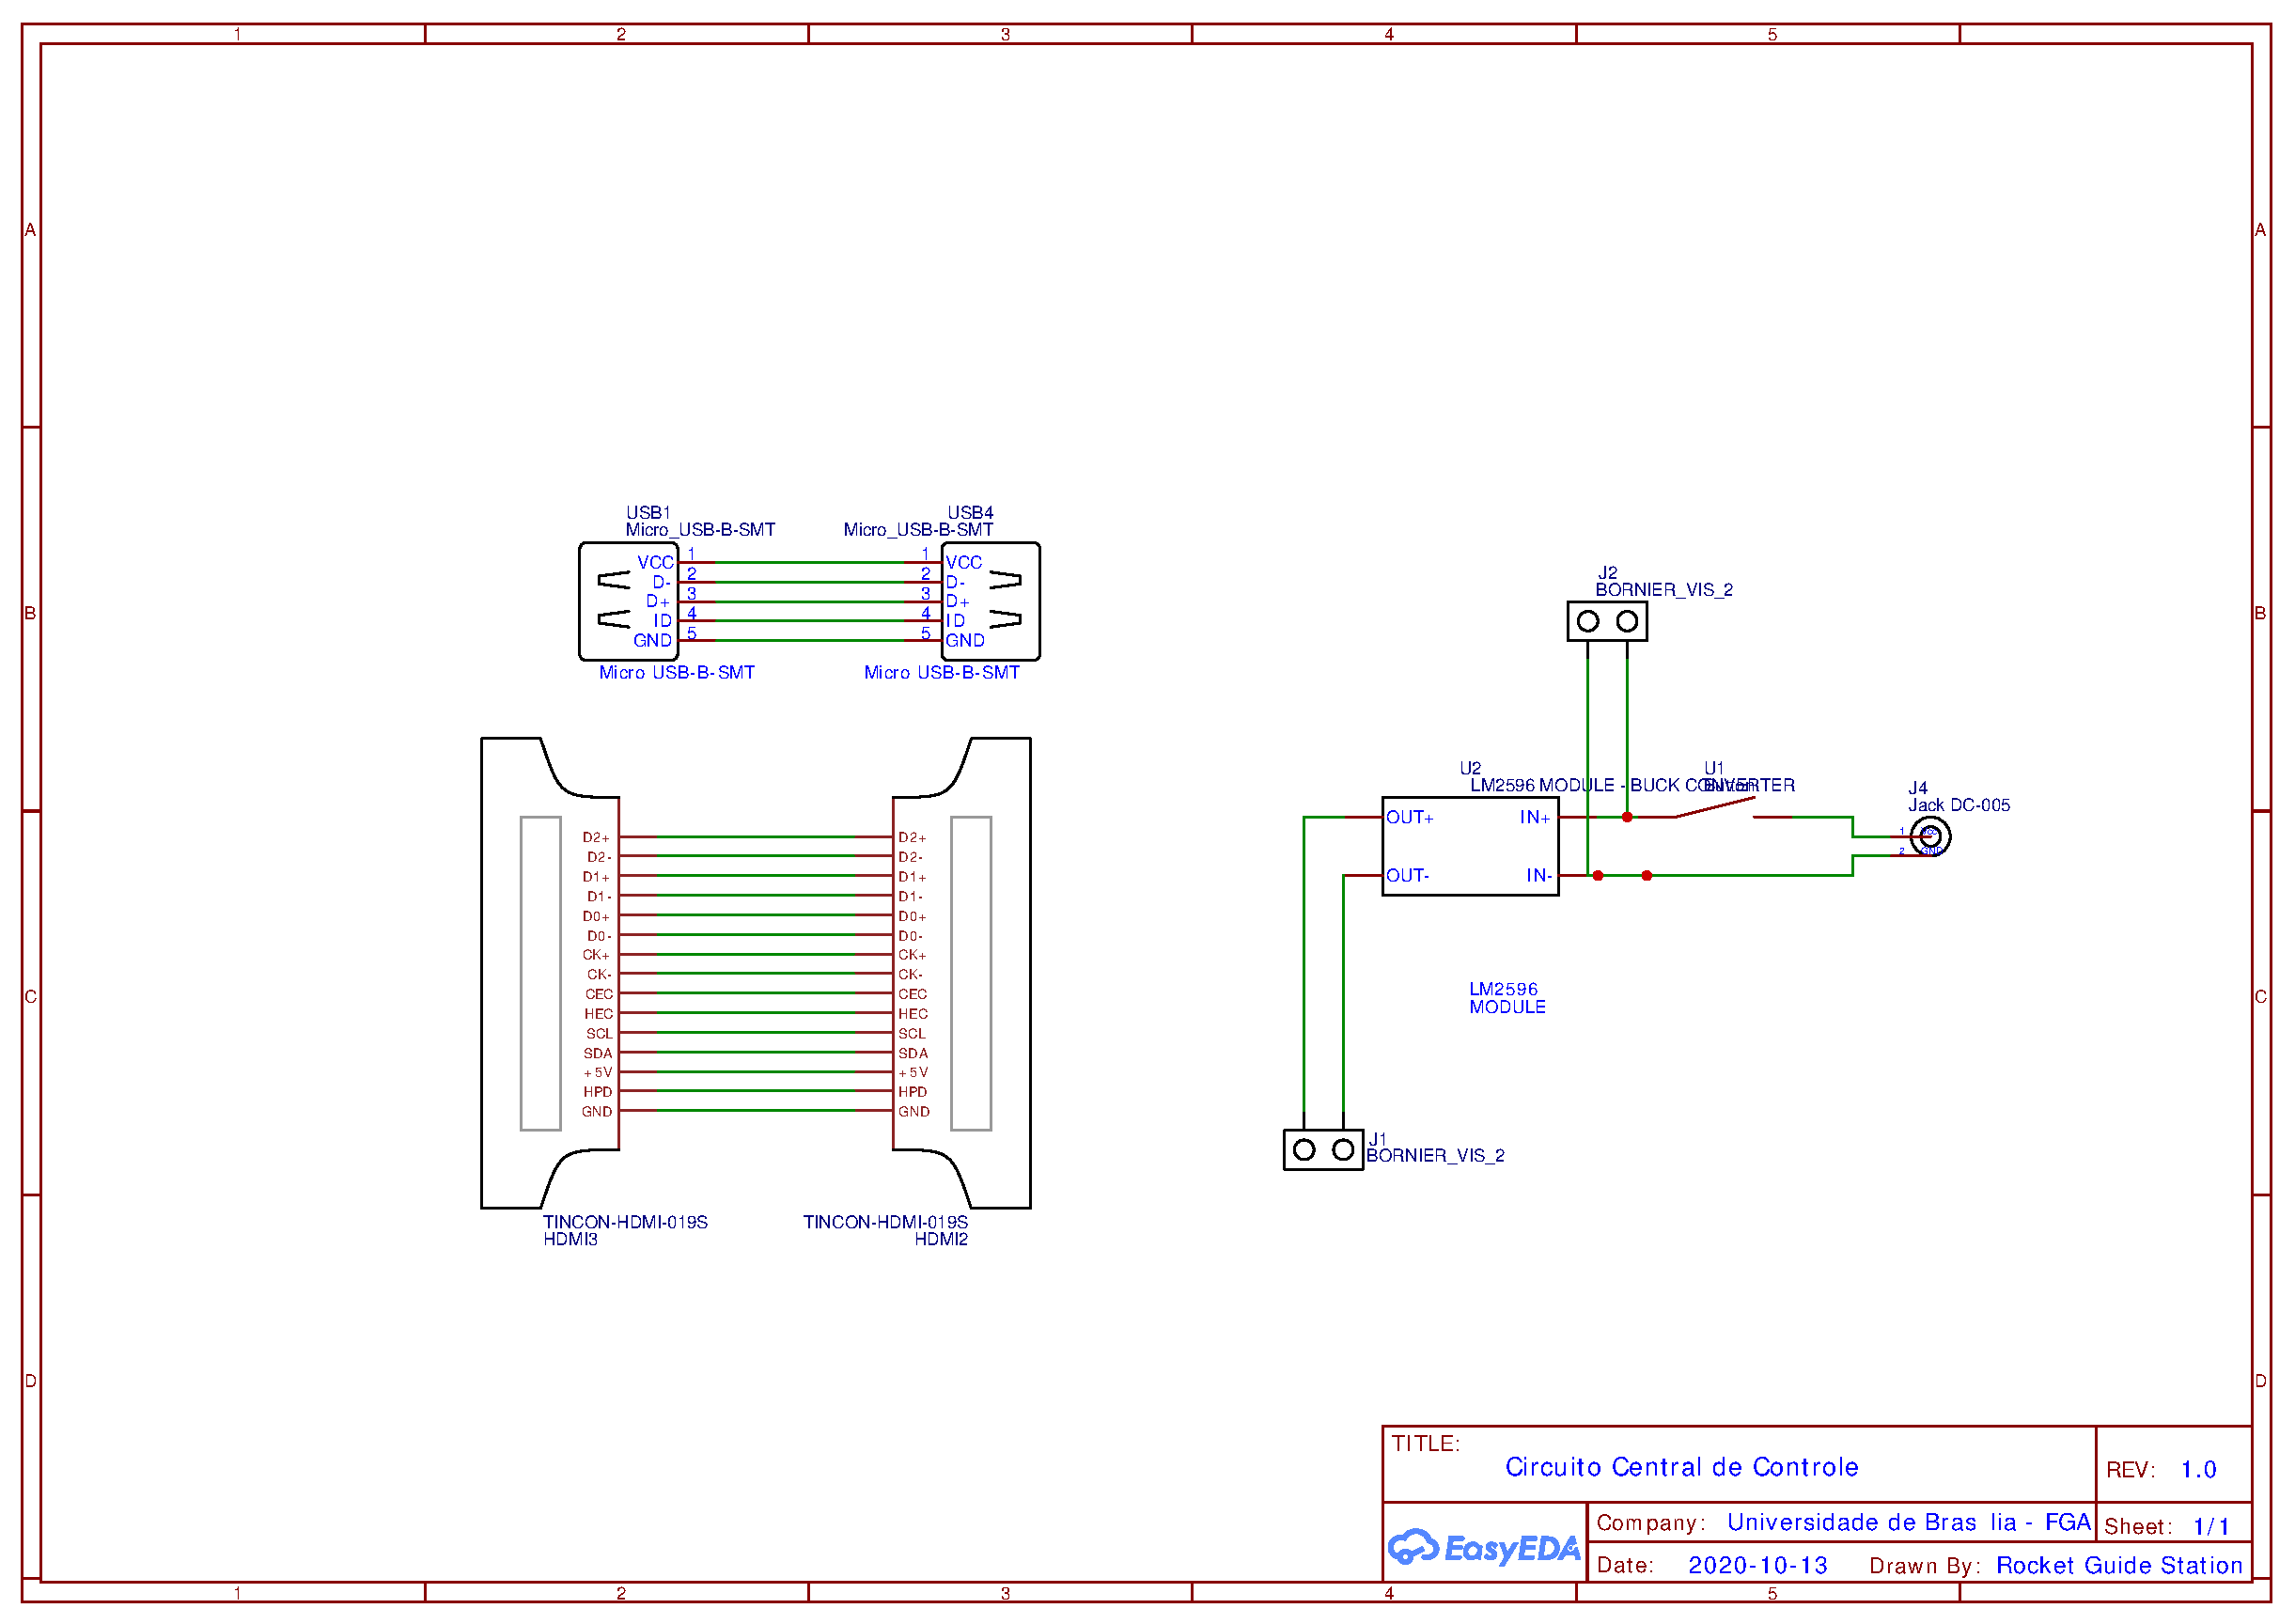
\includegraphics[width=1.3\textwidth, angle=90]{figuras/PDFs/final eletronica/Schematic_maleta final.pdf}
    \caption{Diagrama esquemático circuito da maleta . Fonte: Autor}
    \label{fig:esquematico maleta}
\end{figure}

\begin{figure}[htb]
    \centering
    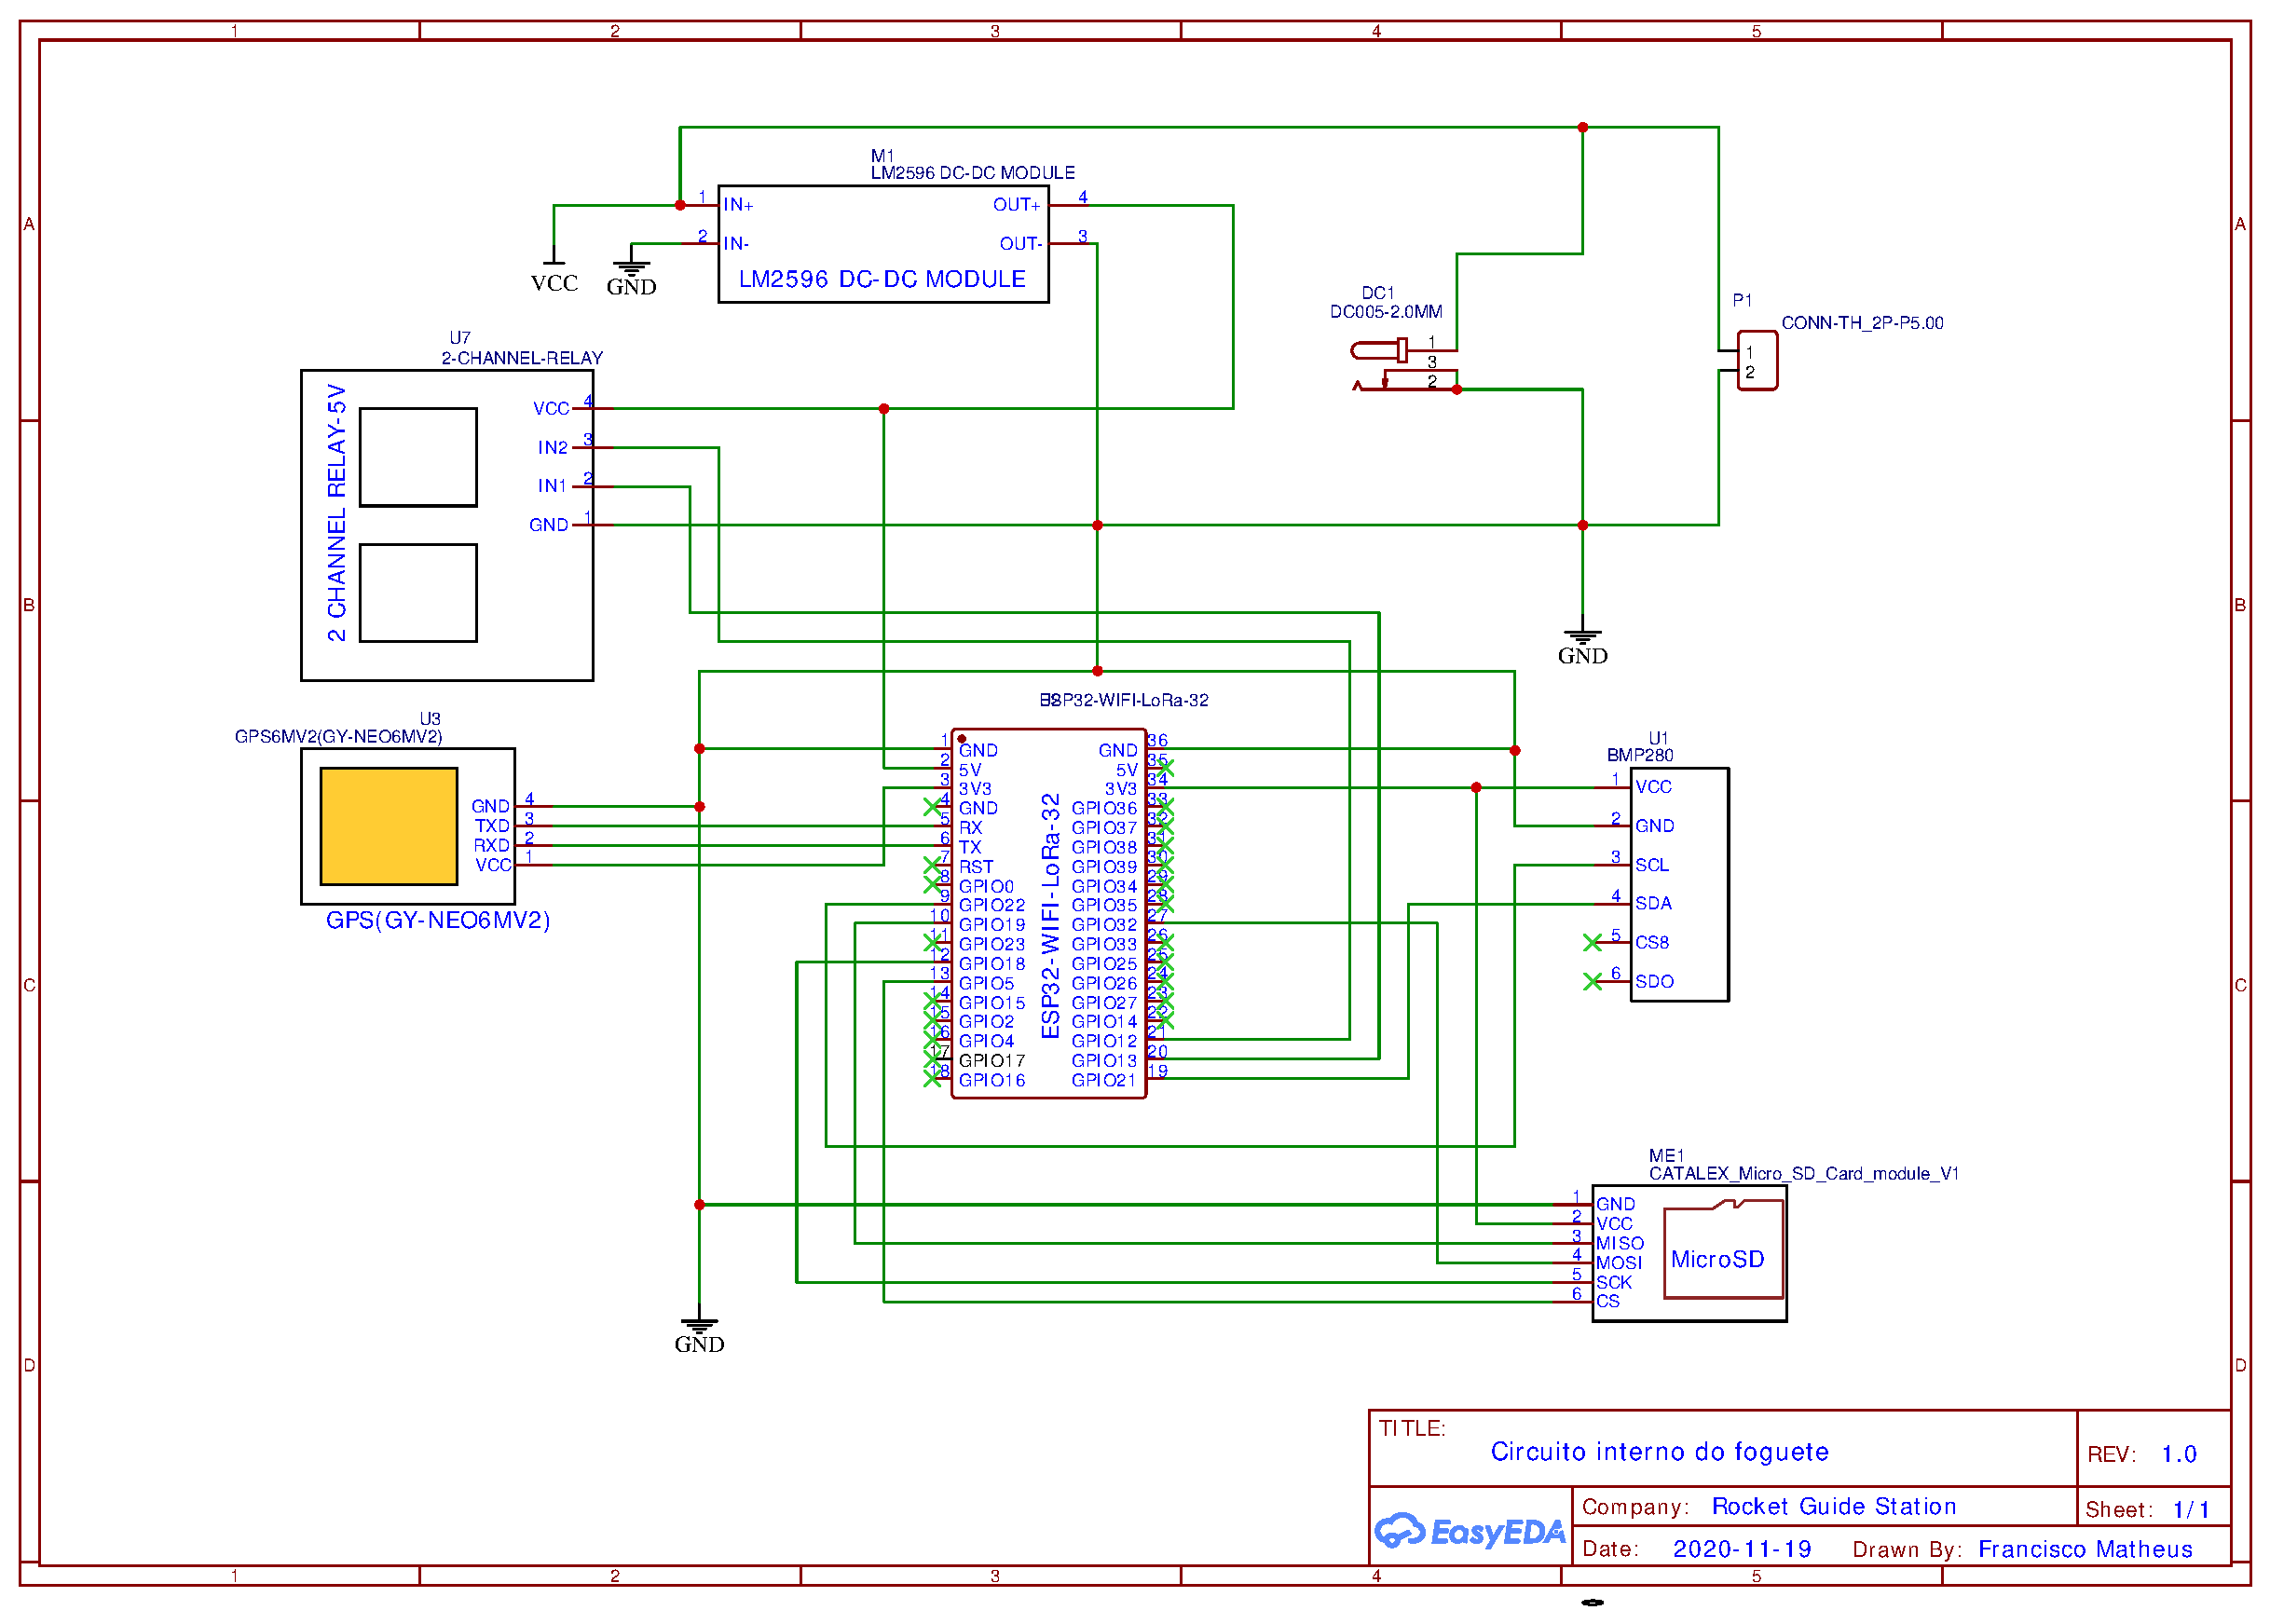
\includegraphics[width=1.3\textwidth, angle=90]{figuras/PDFs/final eletronica/Schematic_Esquemático foguete.pdf}
    \caption{Diagrama esquemático circuito do foguete . Fonte: Autor}
    \label{fig:esquematico foguete}
\end{figure}

\begin{figure}[htb]
    \centering
    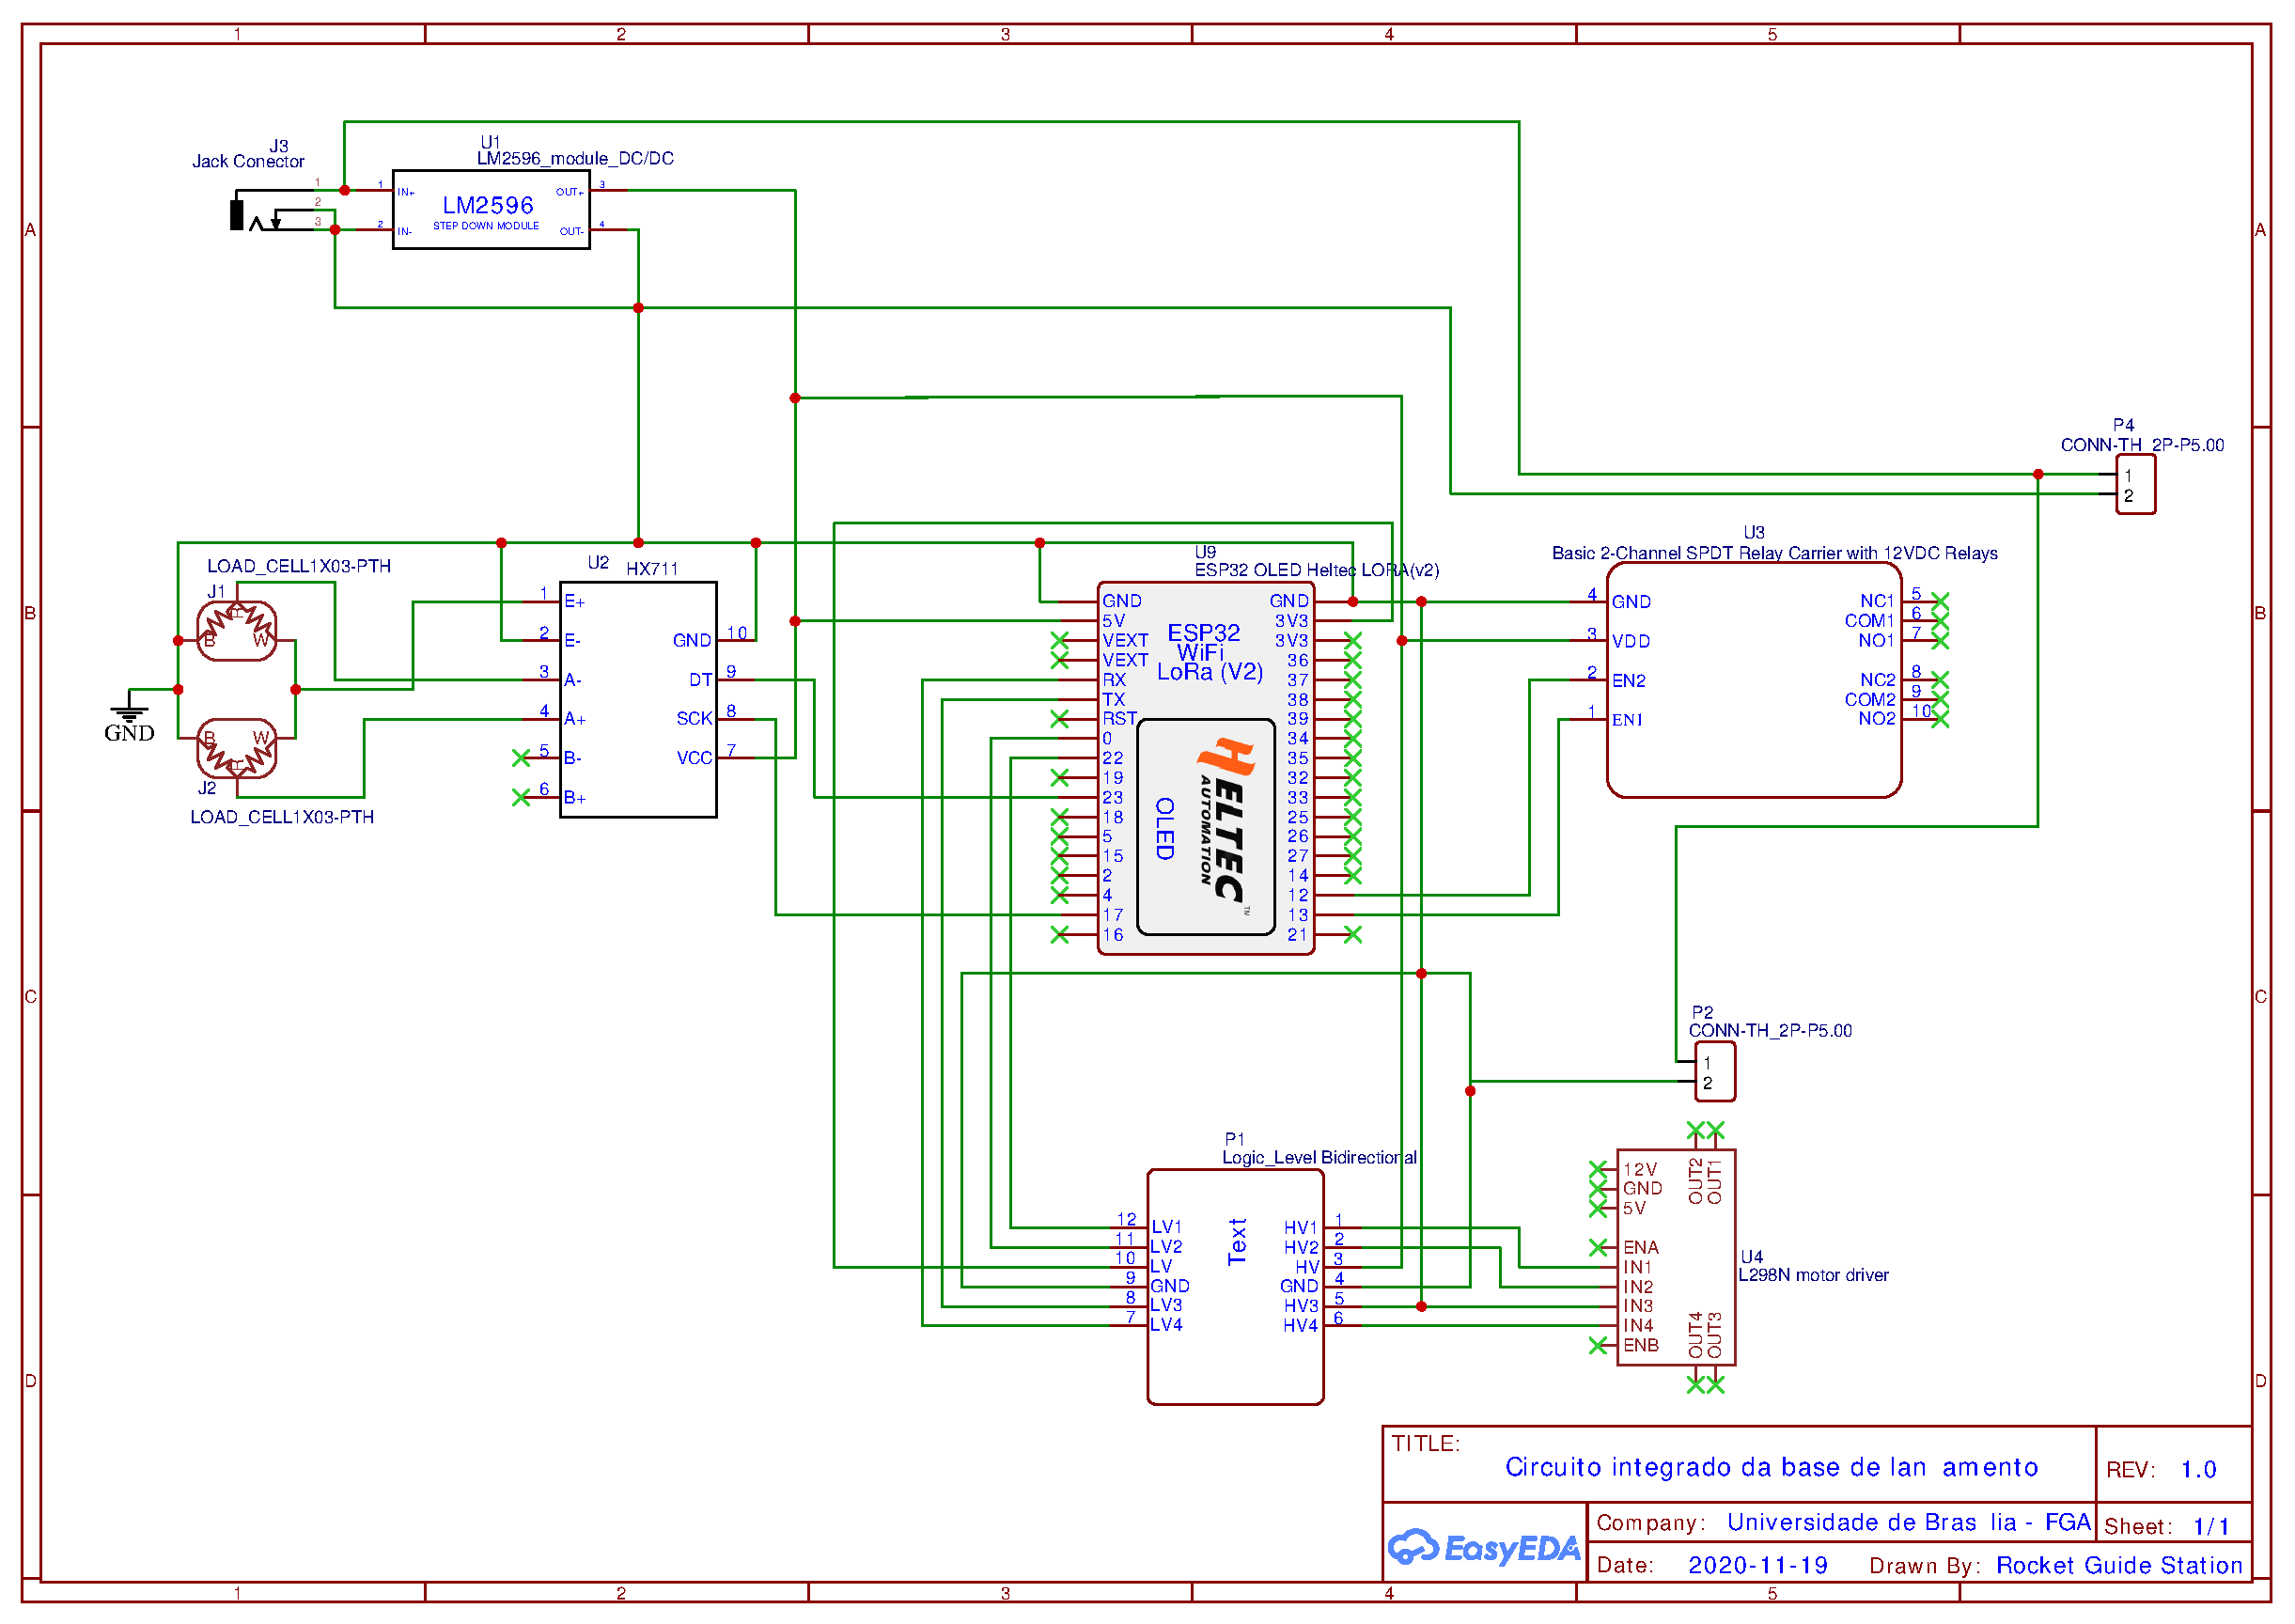
\includegraphics[width=1.3\textwidth, angle=90]{figuras/PDFs/final eletronica/Schematic_base de lançamento.pdf}
    \caption{Diagrama esquemático circuito da base de lançamento . Fonte: Autor}
    \label{fig:esquematico base}
\end{figure}



%\chapter{Diagrama de Blocos/Comunicação}
%\label{Diagrama_Geral}
%\begin{figure}[htb]
 %   \centering
 %   \includegraphics[width=1.1\textwidth, angle=90]{figuras/Diagrama_Geral.png}
  %  \caption{Diagrama de comunicação do projeto. Fonte: Autor}
  %  \url{https://drive.google.com/file/d/12-pXv5L2Z5AuyWWVIr8VZ4WMghu7SYDw/view?usp=sharing}
  %  \label{fig:Diagrama_Geral}
%\end{figure}


\chapter{Diagramas elétricos}
\label{diag_eletrico}

\begin{figure}[H]
    \centering
    \includegraphics[width=1.3\textwidth, angle=270]{figuras/1_diagrama_bifilar_da_maleta.png}
    \caption{Diagrama bifilar GCS}
    \label{fig:diagrama_bifilar_01}
\end{figure}

\begin{figure}[H]
    \centering
    \includegraphics[width=1.3\textwidth, angle=270]{figuras/1_diagrama_bifilar_base_de_lançamento.png}
    \caption{Diagrama bifilar da base de lançamento}
    \label{fig:diagrama_bifilar_02}
\end{figure}

\begin{figure}[H]
    \centering
    \includegraphics[width=1.3\textwidth, angle=270]{figuras/1_diagrama_unifilar_do_sistema_de_carregamento.png}
    \caption{Diagrama unifilar do sistema de carregamento.}
    \label{fig:diagrama_unifilar_01}
\end{figure}

\includepdf[pages=-, angle=270]{figuras/circuitoeletrico.pdf}


\chapter{Esboço e CAD iniciais}
\label{CAD}

\begin{figure}[htb]
    \centering
    \includegraphics[width=0.5\textwidth , angle=90 ]{figuras/EsboçoInicial_V_1.jpg}
    \caption{Esboço inicial}
    \label{fig:esboço}
\end{figure}

\begin{figure} [H]
\centering
  \subfigure[aberto]{
    \includegraphics[width=7cm]{figuras/Back1.PNG}
  } 
  \subfigure[fechado]{ 
    \includegraphics[width=7cm]{figuras/Back2.PNG}
  } 
  \caption{CAD da maleta verso}
\end{figure}

\begin{figure} [H]
\centering
  \subfigure[aberto]{
    \includegraphics[width=7cm]{figuras/Front1.PNG}
  } 
  \subfigure[fechado]{ 
    \includegraphics[width=7cm]{figuras/Front2.PNG}
  } 
  \caption{CAD's da maleta frente}
\end{figure}

\begin{figure} [H]
\centering
  \subfigure[aberto]{
    \includegraphics[width=7cm]{figuras/Lateral1.PNG}
  } 
  \subfigure[fechado]{ 
    \includegraphics[width=7cm]{figuras/Lateral2.PNG}
  } 
  \caption{CAD's da maleta lateral}
\end{figure}

\begin{figure} [H]
\centering
  \subfigure[aberto]{
    \includegraphics[width=7cm]{figuras/Sup1.PNG}
  } 
  \subfigure[fechado]{ 
    \includegraphics[width=7cm]{figuras/Sup2.PNG}
  } 
  \caption{CAD's da maleta superior}
\end{figure}

\begin{figure} [H]
\centering
  \subfigure[aberto]{
    \includegraphics[width=7cm]{figuras/Iso1.PNG}
  } 
  \subfigure[fechada]{ 
    \includegraphics[width=7cm]{figuras/Iso2.PNG}
  } 
  \caption{CAD's da maleta isométrica}
\end{figure}


\chapter{Desenhos Técnicos}
\label{Drafts_do_projeto}

%\section{GCS}

%\includepdf[pages=-,angle=270]{figuras/cad/}



%\includepdf[pages=-]{figuras/cad/}


%\section{MaletaAbastecimento}

\includepdf[pages=-]{figuras/cad/DESENHOTECNICOMALETAALIMENTACAO.pdf}

\includepdf[pages=-]{figuras/cad/DESENHOTECNICOMALETAALIMENTACAO2.pdf}

\includepdf[pages=-,angle=270]{figuras/cad/DESENHOTECNICOMALETAGCS1.pdf}

\includepdf[pages=-,angle=270]{figuras/cad/DESENHOTECNICOMALETAGCS.pdf}

\includepdf[pages=-,angle=270]{figuras/cad/DESENHOTECNICOMALETAGCS2.pdf}

\includepdf[pages=-,angle=270]{figuras/cad/DESENHO TECNICO CASE ELETRONICA.pdf}

\includepdf[pages=-,angle=270]{figuras/cad/DESENHOTECNICO CARREGADOR.pdf}

\includepdf[pages=-,angle=270]{figuras/cad/LISTA DE MATERIAIS GCS.pdf}

\includepdf[pages=-,angle=270]{figuras/cad/TABELA DE MATERIAIS ALIMENTACAO.pdf}

\includepdf[pages=-,angle=270]{figuras/cad/TabelaDeComponenteGCS.pdf}





\chapter{Simulação de Impacto}
\label{simulacoes_impacto}

\begin{figure}[htb]
    \centering
    \includegraphics[width=1.0\textwidth, angle=0]{figuras/estrutura_simulacaoImpacto/ignicaoNormalYLadoMaior.png}
    \caption{Tensão normal no eixo Y da maleta do sistema de alimentação em queda direta}
    \label{fig:simulacaoImpacto_01}
\end{figure}

\begin{figure}[htb]
    \centering
    \includegraphics[width=1.0\textwidth, angle=0]{figuras/estrutura_simulacaoImpacto/ignicaoNormalYLadoMenor.png}
    \caption{Tensão normal no eixo Y da maleta do sistema de alimentação em queda lateral}
    \label{fig:simulacaoImpacto_02}
\end{figure}

\begin{figure}[htb]
    \centering
    \includegraphics[width=1.0\textwidth, angle=0]{figuras/estrutura_simulacaoImpacto/ignicaoNormalYCanto.png}
    \caption{Tensão normal no eixo Y da maleta do sistema de alimentação em queda inclinada}
    \label{fig:simulacaoImpacto_03}
\end{figure}


\begin{figure}[htb]
    \centering
    \includegraphics[width=1.0\textwidth, angle=0]{figuras/estrutura_simulacaoImpacto/ignicaoCisalhamentoXZLadoMaior.png}
    \caption{Tensão de Cisalhamento no plano XZ da maleta do sistema de alimentação em queda direta}
    \label{fig:simulacaoImpacto_04}
\end{figure}

\begin{figure}[htb]
    \centering
    \includegraphics[width=1.0\textwidth, angle=0]{figuras/estrutura_simulacaoImpacto/ignicaoCisalhamentoXZLadoMenor.png}
    \caption{Tensão de Cisalhamento no plano XZ da maleta do sistema de alimentação em queda lateral}
    \label{fig:simulacaoImpacto_05}
\end{figure}

\begin{figure}[htb]
    \centering
    \includegraphics[width=1.0\textwidth, angle=0]{figuras/estrutura_simulacaoImpacto/ignicaoCisalhamentoXZCanto.png}
    \caption{Tensão de Cisalhamento no plano XZ da maleta do sistema de alimentação em queda inclinada}
    \label{fig:simulacaoImpacto_06}
\end{figure}

\begin{figure}[htb]
    \centering
    \includegraphics[width=1.0\textwidth, angle=0]{figuras/estrutura_simulacaoImpacto/ignicaoDeformacaoLadoMaior.png}
    \caption{Deformação da maleta do sistema de alimentação em queda direta}
    \label{fig:simulacaoImpacto_07}
\end{figure}

\begin{figure}[htb]
    \centering
    \includegraphics[width=1.0\textwidth, angle=0]{figuras/estrutura_simulacaoImpacto/ignicaoDeformacaoLadoMenor.png}
    \caption{Deformação da maleta do sistema de alimentação em queda lateral}
    \label{fig:simulacaoImpacto_08}
\end{figure}

\begin{figure}[htb]
    \centering
    \includegraphics[width=1.0\textwidth, angle=0]{figuras/estrutura_simulacaoImpacto/ignicaoDeformacaoCanto.png}
    \caption{Deformação da maleta do sistema de alimentação em queda inclinada}
    \label{fig:simulacaoImpacto_09}
\end{figure}

\begin{figure}[htb]
    \centering
    \includegraphics[width=1.0\textwidth, angle=0]{figuras/estrutura_simulacaoImpacto/ignicaoRevestidaNormalYMaior.png}
    \caption{Tensão normal no eixo Y da maleta do sistema de alimentação revestida em queda direta}
    \label{fig:simulacaoImpacto_10}
\end{figure}

\begin{figure}[htb]
    \centering
    \includegraphics[width=1.0\textwidth, angle=0]{figuras/estrutura_simulacaoImpacto/ignicaoRevestidaNormalYMenor.png}
    \caption{Tensão normal no eixo Y da maleta do sistema de alimentação revestida em queda lateral}
    \label{fig:simulacaoImpacto_11}
\end{figure}

\begin{figure}[htb]
    \centering
    \includegraphics[width=1.0\textwidth, angle=0]{figuras/estrutura_simulacaoImpacto/ignicaoRevestidaNormalYCanto.png}
    \caption{Tensão normal no eixo Y da maleta do sistema de alimentação revestida em queda inclinada}
    \label{fig:simulacaoImpacto_12}
\end{figure}

\begin{figure}[htb]
    \centering
    \includegraphics[width=1.0\textwidth, angle=0]{figuras/estrutura_simulacaoImpacto/ignicaoRevestidaCisalhamentoXZMaior.png}
    \caption{Tensão de cisalhamento no plano XZ da maleta do sistema de alimentação revestida em queda direta}
    \label{fig:simulacaoImpacto_13}
\end{figure}

\begin{figure}[htb]
    \centering
    \includegraphics[width=1.0\textwidth, angle=0]{figuras/estrutura_simulacaoImpacto/ignicaoRevestidaCisalhamentoXZMenor.png}
    \caption{Tensão de cisalhamento no plano XZ da maleta do sistema de alimentação revestida em queda lateral}
    \label{fig:simulacaoImpacto_14}
\end{figure}

\begin{figure}[htb]
    \centering
    \includegraphics[width=1.0\textwidth, angle=0]{figuras/estrutura_simulacaoImpacto/ignicaoRevestidaCisalhamentoXZCanto.png}
    \caption{Tensão de cisalhamento no plano XZ da maleta do sistema de alimentação revestida em queda inclinada}
    \label{fig:simulacaoImpacto_15}
\end{figure}

\begin{figure}[htb]
    \centering
    \includegraphics[width=1.0\textwidth, angle=0]{figuras/estrutura_simulacaoImpacto/ignicaoRevestidaDeformacaoMaior.png}
    \caption{Deformação da maleta do sistema de alimentação revestida em queda direta}
    \label{fig:simulacaoImpacto_16}
\end{figure}

\begin{figure}[htb]
    \centering
    \includegraphics[width=1.0\textwidth, angle=0]{figuras/estrutura_simulacaoImpacto/ignicaoRevestidaDeformacaoMenor.png}
    \caption{Deformação da maleta do sistema de alimentação revestida em queda lateral}
    \label{fig:simulacaoImpacto_17}
\end{figure}

\begin{figure}[htb]
    \centering
    \includegraphics[width=1.0\textwidth, angle=0]{figuras/estrutura_simulacaoImpacto/ignicaoRevestidaDeformacaoCanto.png}
    \caption{Deformação da maleta do sistema de alimentação revestida em queda inclinada}
    \label{fig:simulacaoImpacto_18}
\end{figure}

\begin{figure}[htb]
    \centering
    \includegraphics[width=1.0\textwidth, angle=0]{figuras/estrutura_simulacaoImpacto/maletaNormalYMaior.png}
    \caption{Tensão normal no eixo Y da maleta do sistema de controle em queda direta}
    \label{fig:simulacaoImpacto_19}
\end{figure}

\begin{figure}[htb]
    \centering
    \includegraphics[width=1.0\textwidth, angle=0]{figuras/estrutura_simulacaoImpacto/maletaNormalYMenor.png}
    \caption{Tensão normal no eixo Y da maleta do sistema de controle em queda lateral}
    \label{fig:simulacaoImpacto_20}
\end{figure}

\begin{figure}[htb]
    \centering
    \includegraphics[width=1.0\textwidth, angle=0]{figuras/estrutura_simulacaoImpacto/maletaNormalYCanto.png}
    \caption{Tensão normal no eixo Y da maleta do sistema de controle em queda inclinada}
    \label{fig:simulacaoImpacto_21}
\end{figure}

\begin{figure}[htb]
    \centering
    \includegraphics[width=1.0\textwidth, angle=0]{figuras/estrutura_simulacaoImpacto/maletaCisalhamentoXZMaior.png}
    \caption{Tensão de cisalhamento no plano XZ da maleta do sistema de controle em queda direta}
    \label{fig:simulacaoImpacto_22}
\end{figure}

\begin{figure}[htb]
    \centering
    \includegraphics[width=1.0\textwidth, angle=0]{figuras/estrutura_simulacaoImpacto/maletaCisalhamentoXZMenor.png}
    \caption{Tensão de cisalhamento no plano XZ da maleta do sistema de controle em queda lateral}
    \label{fig:simulacaoImpacto_23}
\end{figure}

\begin{figure}[htb]
    \centering
    \includegraphics[width=1.0\textwidth, angle=0]{figuras/estrutura_simulacaoImpacto/maletaCisalhamentoXZCanto.png}
    \caption{Tensão de cisalhamento no plano XZ da maleta do sistema de controle em queda inclinada}
    \label{fig:simulacaoImpacto_24}
\end{figure}

\begin{figure}[htb]
    \centering
    \includegraphics[width=1.0\textwidth, angle=0]{figuras/estrutura_simulacaoImpacto/maletaDeformacaoMaior.png}
    \caption{Deformação da maleta do sistema de controle em queda direta}
    \label{fig:simulacaoImpacto_25}
\end{figure}

\begin{figure}[htb]
    \centering
    \includegraphics[width=1.0\textwidth, angle=0]{figuras/estrutura_simulacaoImpacto/maletaDeformacaoMenor.png}
    \caption{Deformação da maleta do sistema de controle em queda lateral}
    \label{fig:simulacaoImpacto_26}
\end{figure}

\begin{figure}[htb]
    \centering
    \includegraphics[width=1.0\textwidth, angle=0]{figuras/estrutura_simulacaoImpacto/maletaDeformacaoCanto.png}
    \caption{Deformação da maleta do sistema de controle em queda inclinada}
    \label{fig:simulacaoImpacto_27}
\end{figure}

\begin{figure}[htb]
    \centering
    \includegraphics[width=1.0\textwidth, angle=0]{figuras/estrutura_simulacaoImpacto/maletaRevestidaNormalYMaior.png}
    \caption{Tensão normal Y da maleta revestida do sistema de controle em queda direta}
    \label{fig:simulacaoImpacto_28}
\end{figure}

\begin{figure}[htb]
    \centering
    \includegraphics[width=1.0\textwidth, angle=0]{figuras/estrutura_simulacaoImpacto/maletaRevestidaNormalYMenor.png}
    \caption{Tensão normal Y da maleta revestida do sistema de controle em queda lateral}
    \label{fig:simulacaoImpacto_29}
\end{figure}

\begin{figure}[htb]
    \centering
    \includegraphics[width=1.0\textwidth, angle=0]{figuras/estrutura_simulacaoImpacto/maletaRevestidaNormalYCanto.png}
    \caption{Tensão normal Y da maleta revestida do sistema de controle em queda inclinada}
    \label{fig:simulacaoImpacto_30}
\end{figure}

\begin{figure}[htb]
    \centering
    \includegraphics[width=1.0\textwidth, angle=0]{figuras/estrutura_simulacaoImpacto/maletaRevestidaCisalhamentoXZMaior.png}
    \caption{Tensão de cisalhamento no plano XZ da maleta revestida do sistema de controle em queda direta}
    \label{fig:simulacaoImpacto_31}
\end{figure}

\begin{figure}[htb]
    \centering
    \includegraphics[width=1.0\textwidth, angle=0]{figuras/estrutura_simulacaoImpacto/maletaRevestidaCisalhamentoXZMenor.png}
    \caption{Tensão de cisalhamento no plano XZ da maleta revestida do sistema de controle em queda lateral}
    \label{fig:simulacaoImpacto_32}
\end{figure}

\begin{figure}[htb]
    \centering
    \includegraphics[width=1.0\textwidth, angle=0]{figuras/estrutura_simulacaoImpacto/maletaRevestidaCisalhamentoXZCanto.png}
    \caption{Tensão de cisalhamento no plano XZ da maleta revestida do sistema de controle em queda inclinada}
    \label{fig:simulacaoImpacto_33}
\end{figure}

\begin{figure}[htb]
    \centering
    \includegraphics[width=1.0\textwidth, angle=0]{figuras/estrutura_simulacaoImpacto/maletaRevestidaDeformationMaior.png}
    \caption{Deformação da maleta revestida do sistema de controle em queda direta}
    \label{fig:simulacaoImpacto_34}
\end{figure}

\begin{figure}[htb]
    \centering
    \includegraphics[width=1.0\textwidth, angle=0]{figuras/estrutura_simulacaoImpacto/maletaRevestidaDeformacaoMenor.png}
    \caption{Deformação da maleta revestida do sistema de controle em queda lateral}
    \label{fig:simulacaoImpacto_35}
\end{figure}

\begin{figure}[htb]
    \centering
    \includegraphics[width=1.0\textwidth, angle=0]{figuras/estrutura_simulacaoImpacto/maletaRevestidaDeformacaoCanto.png}
    \caption{Deformação da maleta revestida do sistema de controle em queda inclinada}
    \label{fig:simulacaoImpacto_36}
\end{figure}

\chapter[Registro de alterações]{Registro de alterações}
\label{alteracoes}


\begin{table}[H]
\centering
\begin{tabular}{|l|l|}
\hline
PC2 & \begin{tabular}[c]{@{}l@{}}Estudo sobre as dificuldades de aplicar Aprendizado de Máquina \\ no projeto.\end{tabular} \\ \hline
Seção \ref{Peso_do_Foguete} &  \begin{tabular}[c]{@{}l@{}}Adição de mais uma célula de carga para medição do peso do \\ foguete.\end{tabular}\\ \hline
Seção \ref{sec:baterias} &  \begin{tabular}[c]{@{}l@{}}Uso de duas baterias separadas. \end{tabular}\\ \hline
Seção \ref{sec:carregador} &  \begin{tabular}[c]{@{}l@{}}Construção de um carregador com estrutura a parte das maletas.\end{tabular}\\ \hline
Seção \ref{sec:mud_est} &  \begin{tabular}[c]{@{}l@{}}Separação das maletas e  construção de duas cases de suporte.\end{tabular}\\ \hline
Seção \ref{subsec:atuador} &  \begin{tabular}[c]{@{}l@{}}Válvula esfera selecionada e adaptador para a mesma.\end{tabular}\\ \hline


\end{tabular}
\caption{Lista de alterações significativas do projeto.}
\label{alteracoes}
\end{table}



\chapter[Autoavaliação]{Autoavaliação}
%\addcontentsline{toc}{chapter}{Contextualização}
\label{autoavaliacao}

\begin{itemize}

%    \item \textbf{Nome:Nome}
%    \begin{itemize}
%        \item 
%    \end{itemize}
    
    \item \textbf{Nome: Augusto Moreno Vilarins}
    \begin{itemize}
    \item Refinamento da definição do produto
    \item Levantamento de requisitos
    \item Storytelling
    \item Protótipo de baixa fidelidade
    \item Wireframe
    \item Reuniões de alinhamento com o cliente
    \item Protótipo de média fidelidade
    \item Auxilio na elaboração do documento do Ponto de Controle 2
    \item Correção das mudanças sugeridas para o documento do ponto de controle 2
    \item Revisão e edição do documento de ponto de controle 3
    \item Manual de usuário
    \item Manual de montagem
    \item Documentação das reuniões com clientes
    \item Preparação do ambiente de desenvolvimento do Front end
    \item Auxílio no desenvolvimento do front end
    \end{itemize}
    
    
    \item \textbf{Nome: Artur Cardoso de Almeida}
    \begin{itemize}
      \item Dimensionamento do case de eletrônica. 
      \item Dimensionamento do carregador de energia.
      \item Redimensionamento da estrutura da Maleta 02 - Abastecimento.
      \item Criação dos CADS das maletas.
      \item Criação do CAD da case de de eletrônica.
      \item Criação do CAD do carregador de energia.
      \item Criação dos desenhos técnicos das estruturas.
      \item Tabela de materiais com vista explodida.
      \item Alinhamento sobre a disposição dos componentes da central de controle com o grupo de eletrônica. 
      \item Integração com o subsistema de eletrônica.
      \item Integração com o subsistema de energia.
      \item Renderização da maleta GCS e da maleta de abastecimento.
      \item Renderização do case de eletrônica
      \item Renderização do carregador de energia.
      \item Renderização do sistema de abastecimento.
      \item Orçamento dos componentes para fabricação da maleta.
      \item Auxilio na definição da solução de acoplamento dos atuadores nas válvulas.
      \item Auxílio na edição e revisão do Ponto de Controle 3.
      \item Auxilio na confecção do manual de montagem.
      \item Auxilio na confecção do manual de usuário.
    \end{itemize}


    \item \textbf{Nome: Diogo Filipe Sens}
    \begin{itemize}
     \item Revisão da simulação de impacto.
     \item Elaboração do plano de montagem das estruturas das duas maletas.
     \item Definição dos elementos de fixação dos componentes estruturais das duas maletas.
     \item elaboração de desenhos que ilustrem a sequência de montagem das duas maletas.
     \item Confecção do manual de montagem sobre a parte estrutural da maleta.
     \item Auxílio na elaboração do \textit{case} de suporte do subsistema válvula + motor + adaptador.
    \end{itemize}

    
    \item \textbf{Nome: Douglas Alves Brandão}
    \begin{itemize}
         \item Definição dos requisitos da estrutura utilizada no protótipo.
         \item Definição dos possíveis materiais a serem utilizados na construção da Ground Station.
         \item Auxílio na elaboração dos CADs da maleta. 
         \item Detalhamento das características dos materiais a serem utilizados na construção da Ground Station.
         \item Auxílio na modelagem do sistema de abastecimento. 
         \item Auxílio na simulação do sistema de abastecimento no software Simulink/Matlab.
         \item Definição dos parâmetros do sistema de abastecimento.
        \item Definição da solução para a abertura de válvulas.
         \item Auxílio na elaboração dos documentos dos Pontos de Controles.
         \item Confecção das instruções para o manual de montagem.
        \item Confecção do manual de montagem.
        \item Confecção dos CADs do sistema de abastecimento.
    \end{itemize}


    \item \textbf{Nome: Gustavo Cavalcante Linhares}
    \begin{itemize}
         \item Gerenciamento e acompanhamento das atividades do grupo de eletrônica 
         \item Detalhamento da solução de integração entre hardware e eletrônica
         \item Alinhamento com os gerentes sobre as soluções tomadas e sobre o desenvolvimento do projeto
         \item Alinhamento entre eletrônica, sub áreas do projeto e o Stakeholder sobre as soluções que possuem impacto no trabalho em mais de um grupo dentro do projeto.
         \item Revisão final dos diagramas esquemático e do projeto de PCI's.
         \item Construção do Manual de montagem no subtópico da montagem dos componentes eletrônicos 
         \item Auxilio na construção do Manual de usuário
         \item Revisão da documentação do PC3 do manual de usuário e manual de montagem
    \end{itemize}
    
    
    \item \textbf{Nome: Francisco Matheus Fernandes Gomes}
    \begin{itemize}
     \item Revisão final dos diagramas esquemático e do projeto de PCI's.
    \item Criação do diagrama de blocos do abastecimento do projeto e no auxilio do diagrama geral.
    \item Auxílio na edição e revisão do Ponto de Controle 3.
    \item Confecção do manual de montagem.
    \item Confecção do manual do usuário.
   \item Levantamento e definição de requisito para o funcionamento da telemetria por Lora na ESP32.
   \item Auxílio na definição da solução de acionamento e controle eletrônico das válvulas internas e externas ao foguete.
    \item Auxílio na integração da eletrônica com os grupos de energia e estrutura.
    \item Atualização dos custos dos componentes que envolve o hardware do projeto.
    \end{itemize}
    
    \item \textbf{Nome: Gabriela Alves da Gama}
    \begin{itemize}
     \item Desenvolvimento do Manter Hardware e Comando;
    \item Configuração do banco de dados;
    \item Desenvolvimento do Manter Foguete;
    \item Desenvolvimento do calculo de velocidade;
    \item Desenvolvimento do manter altitude, gps, missao, peso, pressão, e velocidade; 
    \item Descrever construção do backend;
    \item Desenvolvimento do serviço de simulação
    \item Revisão dos artefatos de software
    \end{itemize}

    
    \item \textbf{Nome: Isaque Alves de Lima}
    \begin{itemize}
    \item Gerenciamento de riscos do projeto;
    \item Direcionamento nas reuniões;
    \item Apoio no alinhamento entre as áreas do projeto;
    \item Edição e revisão do Ponto de Controle 3;
    \item Alinhamento e acompanhamento das atividades do projeto;
    \item Desenvolvimento do Manter Hardware e Comando;
    \item Configuração do banco de dados;
    \item Desenvolvimento do Manter Foguete;
    \item Desenvolvimento do calculo de velocidade;
    \item Desenvolvimento do manter altitude, gps, missao, peso, pressão, e velocidade;
    \item Documentação da API;
    \item Diagrama de pacotes do backend;
    \item Reuniões de alinhamento Software-eletrônica;
    \item Cenários de teste;
    \item Apendice GitHub;
    \item Descrever construção do backend;
    \item Plano de teste do manual de montagem;
    \item Atualização do diagrama de sequência da solução;
    \item Descrever construção do front end;
    \item Atualização das metas e restrições da arquitetura;
    \item Revisão das atividades de software;
    \item Revisão final dos diagramas e imagens;
    \end{itemize}
    
    
    \item \textbf{Nome: João Henrique Egewarth}
    \begin{itemize}
    \item Gerenciamento e acompanhamento das atividades do grupo de software;
    \item Reuniões com clientes;
    \item Descrever construção do front end;
    \item Auxílio na edição e revisão do Ponto de Controle 3;
    \item Alinhamento e acompanhamento das atividades do projeto;
    \item Documentação da API;
    \item Elaboração dos cenários de teste;
    \item Desenvolvimento do Front end da aplicação;
    \item Preparação do ambiente de desenvolvimento do Front end;
    \item Alinhamento com eletrônica para desenvolvimento da comunicação serial;
    \item Diagrama de pacotes do Front end;
    \item Escrita sobre a infraestrutura necessária para a emulação do ambiente com arquitetura computacional Arm64 em ambientes com arquitetura x86;
    \end{itemize}
    
    \item \textbf{Nome: Luísa Prospero de Carvalho silva}
    \begin{itemize} 
     \item Correções levantadas para o documento do ponto de controle.
     \item Revisão e edição do documento de ponto de controle 3
     \item Construção e revisão do Manual de usuário
     \item Construção e revisão do Manual de montagem 
     \item Definição do material para as case.
     \item Definição dos requisitos da estrutura utilizada no protótipo.
     \item Modelagem do sistema de abastecimento. 
     \item Diagrama técnico do sistema de abastecimento.
     \item Gerenciamento e acompanhamento das atividades do grupo de estrutura e energia 
     \item Alinhamento com os gerentes sobre as soluções tomadas e sobre o desenvolvimento do projeto
     \item Revisão final dos desenhos técnicos.
     \item Revisão final de energia e estrutura
     \item Auxílio na definição da solução de acoplamento da válvula e do motor.
     \item Plano de teste do manual de montagem;
     \item Auxilio na definição da solução de acoplamento dos atuadores nas válvulas.
     \item Atualização dos custos dos componentes da estrutura.
     \item caracterização dos componentes de abastecimento
   \end{itemize}
    
    \item \textbf{Nome: Milena Martins Magalhães}
    \begin{itemize}
    \item Elaboração do manual de usuário para operação do sistema de carregamento e  manutenção das baterias.
    \item Elaboração do plano de testes para o sistema de carregamento.
    \item Elaboração do manual de montagem do carregador.
    \item Alinhamento com equipes de estrutura e eletrônica para integração.
    \item Atualização dos custos dos componentes do sistema de alimentação e carregamento.
    \item Confecção da Placa de Circuito Impresso do carregador no EasyEDA.
    \item Auxílio na edição e revisão do documento do Ponto de Controle 3.
    \end{itemize}
    
    
    \item \textbf{Nome: Misael de Souza Andrade}
    \begin{itemize}
    \item Definição da solução de acionamento dos atuadores das válvulas e ignição.
    \item Criação do diagrama de algoritmo da calibração do sensor de peso.
    \item Auxílio na edição e revisão do Ponto de Controle 3.
    \item Confecção do manual de montagem, mais especificamente do subgrupo da Eletrônica.
   \item Levantamento e deificação de requisito para o funcionamento do sensoriamento.
   \item Auxílio na definição da solução de acionamento e controle eletrônico das válvulas internas e externas ao foguete.
   \item Auxílio na definição da solução do pacote de dados transmitidos pela ESP32 LoRa.
   \item Auxílio na integração da eletrônica com os grupos de energia e estrutura.
    \end{itemize}
    
    
    \item \textbf{Nome: Thainá Rodrigues Fernandes}
    \begin{itemize}
    \item Elaboração do manual de usuário para operação do sistema de carregamento e manutenção das baterias.
	\item Elaboração do plano de testes para o sistema de alimentação e do carregador.
	\item Elaboração do manual de montagem do sistema de alimentação da maleta e da base de lançamento.
	\item Alinhamento com equipes de estrutura e eletrônica para integração.
	\item Atualização dos custos dos componentes do sistema de alimentação e carregamento.
	\item Pareamento com outras equipes sobre a solução da ignição.
	\item Atualização dos diagramas unifilares dos sistemas de controle e da base.
	\item Auxílio na edição e revisão do documento do Ponto de Controle 3.
    \end{itemize}

    
    
    
\end{itemize}




\chapter{Manual de Montagem}
\label{Manual_de_montagem}
%\includepdf[pages=-]{editaveis/geral/Manual_de_montagem.pdf}
Enviado separadamente, por questões técnicas.


\chapter{Manual de Usuário}
\label{Manual_de_usuario}
%\includepdf[pages=-]{editaveis/geral/Manual_de_usuario.pdf}
Enviado separadamente, por questões técnicas.


%\chapter{Guia Rápido de instalação do Abastecimento}
%\label{Guia_rapido}
%\includepdf[pages=-]{manuais/guia.pdf}


\end{apendicesenv}

